% Academic rewrite
Geospatial storage and processing in the cloud rest on a set of architectural and representational foundations that this chapter establishes. The cloud-native architectural model provides the setting, placing data in object storage and provisioning compute independently of it \parencite{dageville2016_snowflake_elastic_data_warehouse, pang2024_storage_disaggregated_databases}. Within that setting, geometry and indexing fix how spatial values are represented and how an engine locates the geometries that satisfy a predicate without reading every record, and the spatial data formats and storage models under study determine how those representations are packaged on disk and inside query engines. Distributed spatial processing then describes how a spatial query executes across a shared-nothing cluster at run-time, completing the groundwork on which the formats and engines examined in this thesis are characterized.

\section{Cloud-native data architecture}
\label{background:cloud-native-data-architecture}
\subsection{Decoupled storage and compute} 
\label{background:cloud-native-data-architecture:decoupled-storage-and-compute}
Traditional data processing systems co-locate storage and compute on the same node, each node being a single server in the cluster, so each node processes only the data it stores locally. This tight coupling, the architectural binding of compute and storage to the same hardware, forces the two layers to scale together, even when demand for each grows at different rates \parencite{dageville2016_snowflake_elastic_data_warehouse}.

Cloud architectures decouple these layers, placing data in object storage and provisioning compute, the on-demand allocation of processing capacity, independently of storage, as Figure~\ref{fig:storage-compute-architectures} illustrates. Object storage is a network-accessible store in which each object is identified by a unique key \parencite{calder2011_windows_azure_storage,mesnier2003_object_based_storage}. It is inexpensive and effectively unbounded in capacity, but offers no query capabilities. The separation allows storage and compute to be scaled, priced, and allocated independently \parencite{pang2024_storage_disaggregated_databases}, and compute can be shut down entirely when idle \parencite{dageville2016_snowflake_elastic_data_warehouse}. Multiple engines, software systems that execute queries against the data, can also read the same underlying data without coordinating through a shared server \parencite{pang2024_storage_disaggregated_databases}. \textcite{dageville2016_snowflake_elastic_data_warehouse} note that this arrangement incurs higher latency and \acrfull{cpu} overhead per request than a node in which compute and storage are tightly coupled. This penalty makes format design critical: formats that minimize the volume of data read per query gain a clear advantage.

\begin{figure}[H]
    \centering
    \subfloat[Coupled storage and compute.\label{fig:coupled-compute}]{%
        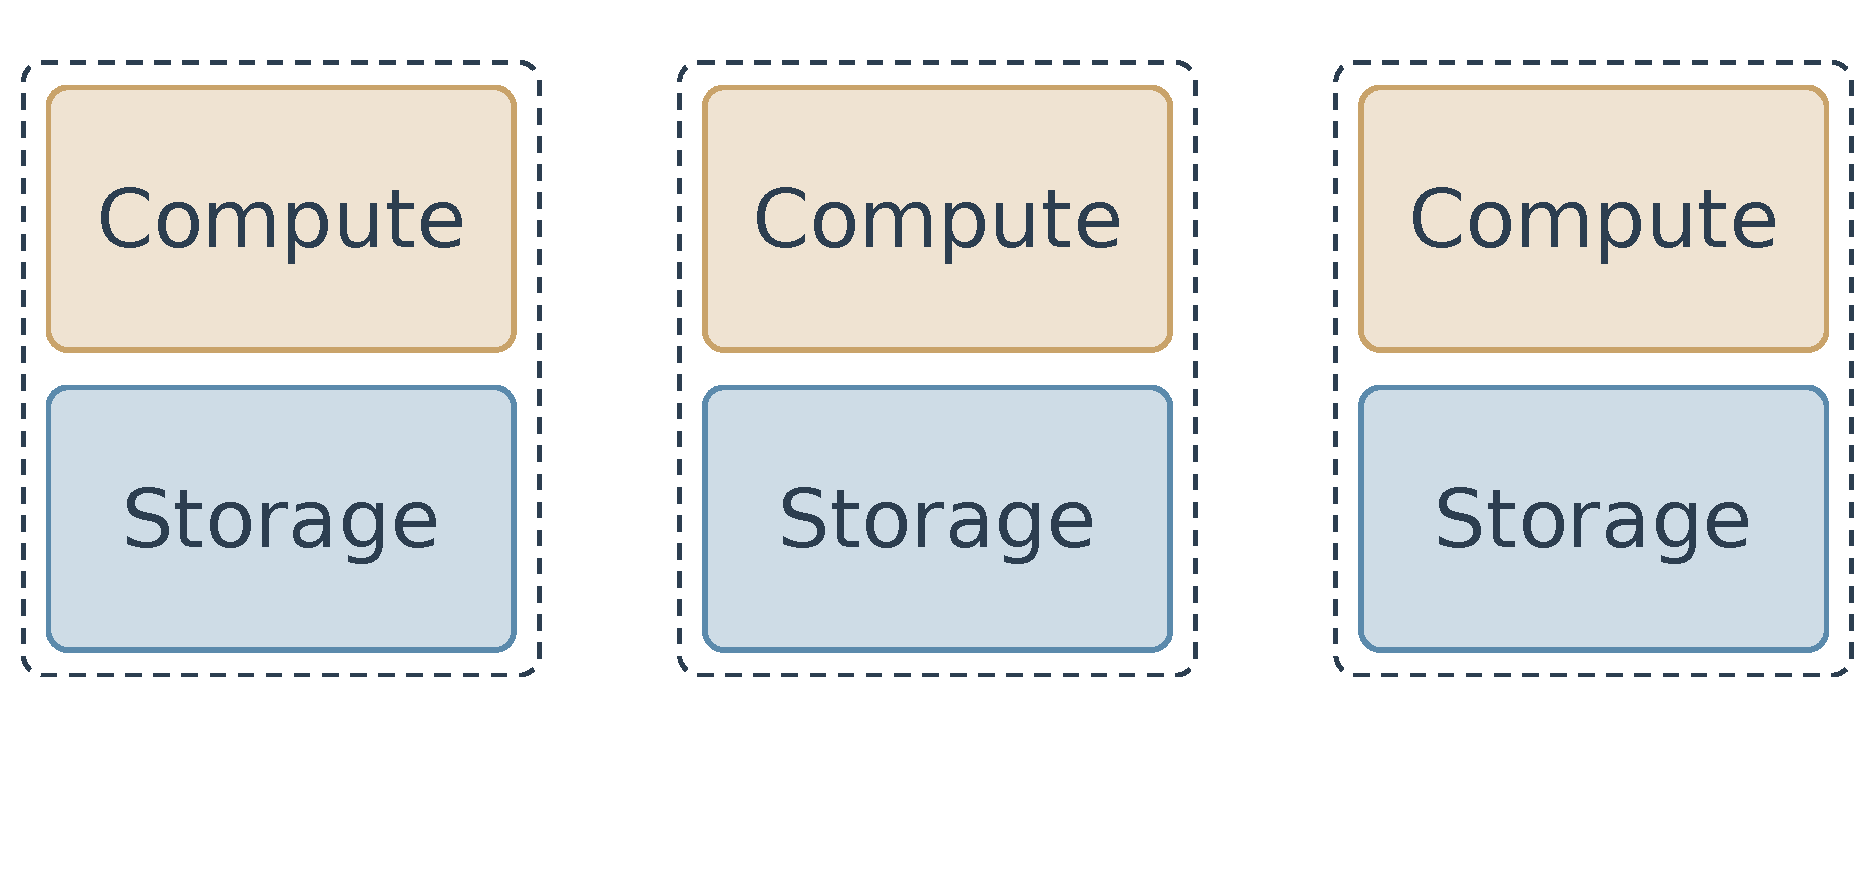
\includegraphics[valign=t, width=0.45\textwidth]{Chapters/02-background/sub-chapters/figures/02-coupled-compute.pdf}%
    }
    \hfill
    \subfloat[Decoupled storage and compute.\label{fig:decoupled-compute}]{%
        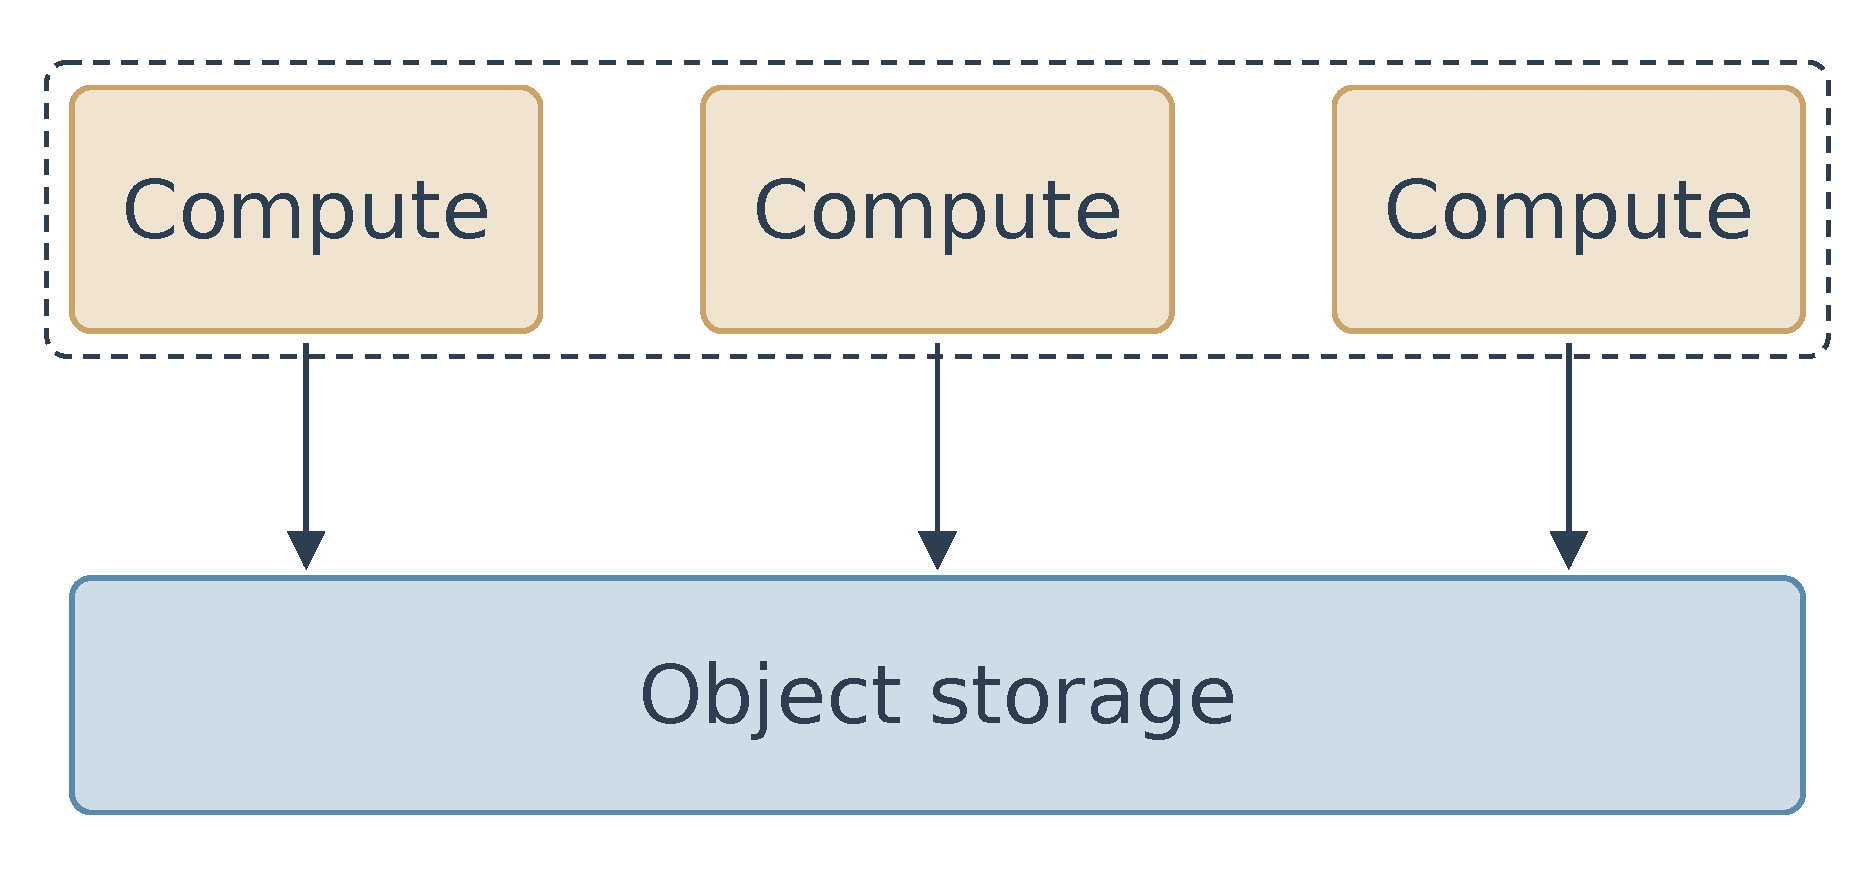
\includegraphics[valign=t, width=0.45\textwidth]{Chapters/02-background/sub-chapters/figures/02-decoupled-compute.pdf}%
    }
    \caption[Coupled versus decoupled storage and compute architectures.]{Comparison of storage and compute architectures. (a) In the traditional coupled architecture, each node bundles its own compute and storage, so the two layers must scale together as a unit. (b) In the decoupled architecture, multiple independent compute resources access a shared object storage layer, allowing storage and compute to be provisioned, priced, and scaled independently of one another.}
    \label{fig:storage-compute-architectures}
\end{figure}

\subsection{Object storage and HTTP access}
\label{background:cloud-native-data-architecture:object-storage-and-http-access}
As the shared layer underlying these architectures, object storage organizes data as opaque objects, byte sequences that the store does not inspect, each identified by a key within a flat container namespace, and serves them through a network \acrfull{api} rather than through the \acrfull{posix} file system calls used for traditional local-disk access \parencite{mesnier2003_object_based_storage, calder2011_windows_azure_storage}. Commercial implementations such as Azure Blob Storage expose each object as an \acrfull{https} \acrfull{url} accessed over \acrfull{http} \parencite{microsoft2024_azure_blob_introduction}.

Read access is mediated by \acrshort{http} itself. \textcite{fielding2022_rfc9110_http_semantics} standardize the \texttt{Range} request header, which allows a client to retrieve an arbitrary byte interval of a remote resource without downloading the whole file. Operational experience confirms the viability of this access model for analytical workloads, queries that scan and aggregate large volumes of data, at scale \parencite{vuppalapati2020_snowflake_elastic_query_engine, durner2023_exploiting_cloud_object_storage}. Cloud-native data formats are designed around this access pattern: layout metadata sits at a fixed byte offset known in advance, so that a reader fetches it first and then issues range requests for only the byte intervals required by the query \parencite{maso2023_ogc_cog_standard}, as Figure~\ref{fig:http-range-requests} illustrates.

\begin{figure}[H]
    \centering
    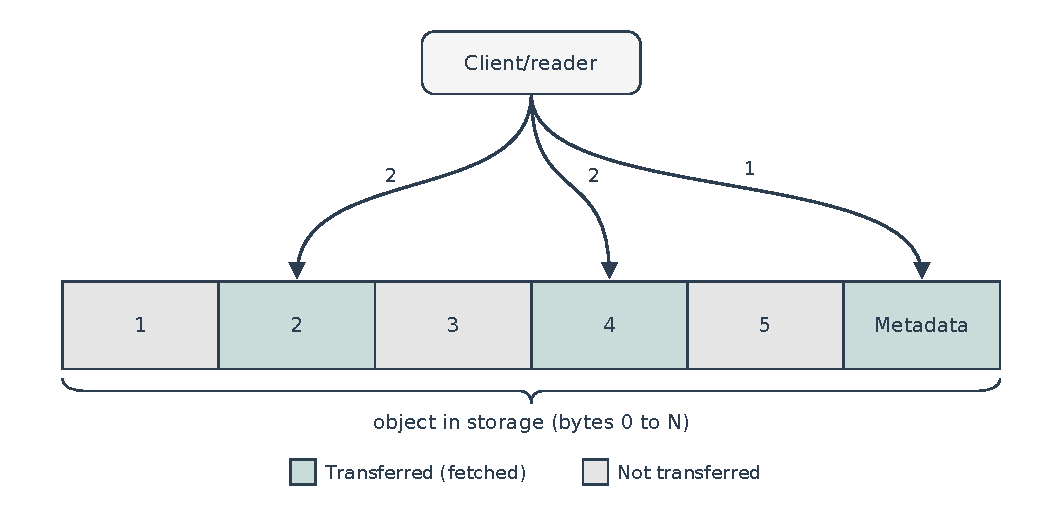
\includegraphics[width=0.85\textwidth]{Chapters/02-background/sub-chapters/figures/02-http-range-requests.pdf}
    \caption[HTTP range request access pattern.]{HTTP range request access pattern for cloud-native objects. The reader first issues a small range request for the metadata block at a known offset within the object (1), parses the layout information it returns to identify which byte intervals satisfy the query, and then issues range requests for only those intervals (2). Bytes outside the requested intervals are never transferred.}
    \label{fig:http-range-requests}
\end{figure}


\subsection{Distributed and non-distributed computation}
\label{background:cloud-native-data-architecture:distributed-and-non-distributed-computation}
With storage and compute decoupled, the choice of computational model becomes a central architectural decision. The non-distributed model runs a query end-to-end inside a single process, an operating-system execution context with its own memory, on one node, and incurs no coordination overhead between workers \parencite{mcsherry2015_scalability_but_at_what_cost}. The distributed model splits both data and computation across multiple worker nodes, where each worker handles a share of the data and runs its assigned tasks, coordinated by a driver or scheduler that dispatches work and aggregates results \parencite{stonebraker1986_case_for_shared_nothing,zaharia2012_resilient_distributed_datasets}. Figure~\ref{fig:compute-models} contrasts the two models.

\begin{figure}[H]
    \centering
    \subfloat[Non-distributed compute.\label{fig:non-distributed-compute}]{%
        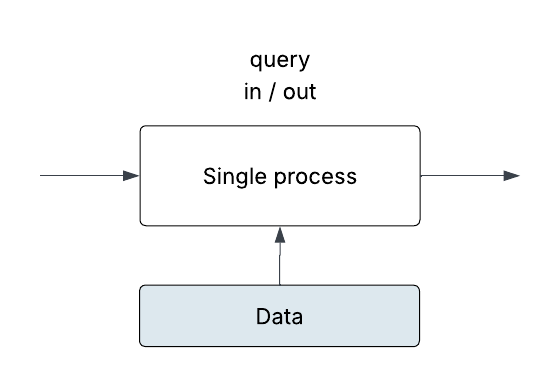
\includegraphics[valign=t, width=0.45\textwidth]{Chapters/02-background/sub-chapters/figures/02-non-distributed-compute.png}%
    }
    \hfill
    \subfloat[Distributed compute.\label{fig:distributed-compute}]{%
        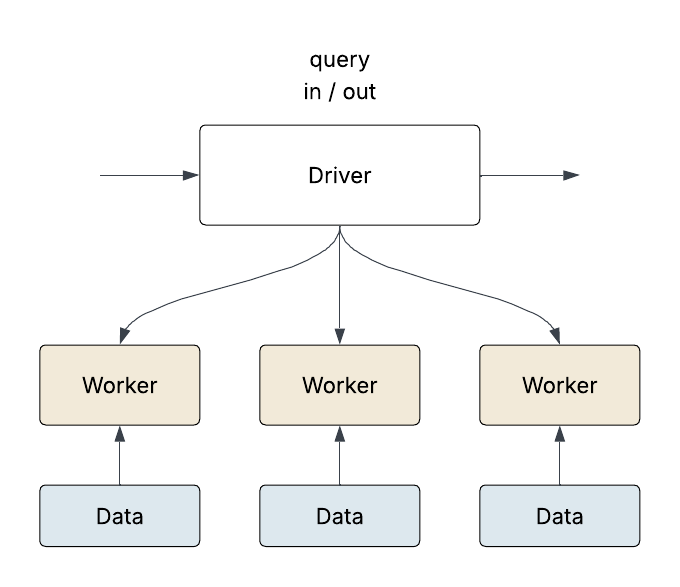
\includegraphics[valign=t, width=0.45\textwidth]{Chapters/02-background/sub-chapters/figures/02-distributed-compute.png}%
    }
    \caption[Non-distributed versus distributed compute models.]{Comparison of compute models. (a) In the non-distributed model, a single process executes the query end-to-end, with no coordination overhead between workers. (b) In the distributed model, a driver dispatches tasks to multiple workers, each operating on a partition of the data.}
    \label{fig:compute-models}
\end{figure}

This distribution introduces overhead from four sources: task scheduling, the assignment of work to specific executors; data shuffling between nodes, the network-based redistribution of intermediate data; serialization of in-memory objects into transmittable byte form; and network communication between workers. Each adds latency before any computation begins \parencite{mcsherry2015_scalability_but_at_what_cost,zaharia2012_resilient_distributed_datasets}. Distributed systems therefore outperform single-node systems only when the dataset or computation is large enough to justify the coordination cost \parencite{mcsherry2015_scalability_but_at_what_cost}. For spatial workloads in particular, the data partitioning strategy is critical: poor spatial partitioning produces skewed workloads, a recognized failure mode in which some workers process far more data than others, so the parallel efficiency, the speedup actually realized from each additional worker, degrades \parencite{tang2020_locationspark_distributed_spatial_query}.

\subsection{Cloud cost model}
\label{background:cloud-native-data-architecture:cloud-cost-model}
The choice between distributed and non-distributed compute is ultimately governed by a cost model in which every resource---storage, processing, and bandwidth---is separately metered \parencite{mell2011_nist_definition_of_cloud_computing}. Pricing follows a pay-as-you-go model: compute and storage are acquired on a short-term basis and released when no longer needed \parencite{armbrust2010_view_of_cloud_computing}. Each resource carries its own pricing dimension. Compute is billed in per-minute increments for allocated virtual cores, the processor units assigned to a workload \parencite{microsoft2024_virtual_machines_pricing}. Object storage is priced per gigabyte-month across access tiers, the storage classes that differ by retrieval frequency and per-GB cost, with transactional \acrshort{api}s, the per-request operations such as reads and writes, charged per \num{10000} operations \parencite{microsoft2024_azure_data_lake_storage_pricing}. Outbound traffic is billed per gigabyte of egress, the traffic leaving the provider's network for the public internet \parencite{microsoft2024_bandwidth_pricing}. To dampen the volatility of on-demand pricing, providers offer reserved instances, prepaid capacity commitments that lock in lower per-hour rates over one- or three-year terms \parencite{microsoft2024_azure_reservations}. Elasticity, the ability to provision and release resources rapidly to match demand \parencite{mell2011_nist_definition_of_cloud_computing}, therefore has direct cost implications: serverless platforms provision compute on a per-request basis and release it automatically when idle, so customers are charged only for active execution time, whereas long-running clusters continue to accrue charges regardless of utilization \parencite{jonas2019_berkeley_view_on_serverless_computing}.
\input{Chapters/02-background/sub-chapters/02-geometry-and-indexing}
\section{Spatial data formats and storage models}
\label{background:spatial-data-formats-and-storage-models}

Spatial data storage spans a spectrum from simple flat files to full database engines. At one end, a format may be a self-contained file that any application can read directly from disk; at the other, the data resides inside a server process that mediates all access through a query language. Between the two sit single-file databases, which embed a query engine in a portable file. An access pattern is the sequence of reads and seeks a workload performs against the data. The choice of tier determines which access patterns the format supports efficiently, how data scales, and whether the format fits the decoupled storage and compute model of cloud architectures \parencite{cngfoundation2024_cloud_optimized_geospatial_formats_guide}. The depth of each treatment tracks its relevance to the benchmark: the Shapefile and GeoParquet formats, the PostGIS and DuckDB engines, and the GeoPandas library are described in full, while the remaining implementations are summarized only enough to delimit each tier and place the evaluated formats within the wider range of options.

\subsection{File formats}
\label{background:spatial-data-formats-and-storage-models:file-formats}
A file format in this context is a self-contained file or bundle of files that encodes spatial data without an accompanying engine. An external library that parses the format is often required to read the data. Typically, the data is read in one of two ways: sequentially, from start to end, or by random access\footnote{Random access denotes reading from an arbitrary position in the file without first traversing the bytes that precede it, in contrast to sequential reading.} at a byte offset, the position measured in bytes from the start of the file. Object storage in cloud environments differs fundamentally from local disk access, since each read operation is an \acrshort{http} request whose per-request latency, the fixed round-trip overhead independent of payload size, runs on the order of tens of milliseconds. This overhead makes patterns that issue many small requests inefficient \parencite{esri2024_cloud_imagery_storage}. Cloud-native file formats address this by structuring the file so that a client can retrieve only the byte intervals it needs through \acrshort{http} range requests, using internal metadata to locate the relevant chunks of data without downloading the entire file \parencite{ogc2023_cog_standard_21026}.

\subsubsection{Shapefile}
\label{background:spatial-data-formats-and-storage-models:file-formats:shapefile}
The Shapefile is a vector data format introduced by \acrfull{esri} in 1998 and remains one of the most widely supported formats in the \acrfull{gis} ecosystem \parencite{esri1998_shapefile_technical_description}. It is not a single file but a bundle sharing a common prefix, with three mandatory files and several optional ones, listed in Table~\ref{tab:shapefile-components}.

\begin{table}[H]
    \centering
    \caption[Shapefile component files]{Mandatory and optional files in the Shapefile format.}
    \label{tab:shapefile-components}
    \begin{tabular}{lll}
        \toprule
        \textbf{Extension} & \textbf{Type} & \textbf{Content} \\
        \midrule
        \texttt{.shp} & Mandatory & Variable-length geometry records \\
        \texttt{.shx} & Mandatory & Record indexes \\
        \texttt{.dbf} & Mandatory & Feature attributes (dBASE table) \\
        \texttt{.prj} & Optional & \acrlong{crs} (\acrshort{wkt}) \\
        \texttt{.sbn} / \texttt{.sbx} & Optional & Spatial index (\acrshort{esri}, undocumented) \\
        \texttt{.qix} & Optional & Spatial index (quadtree, open-source) \\
        \bottomrule
    \end{tabular}
\end{table}

The three mandatory files are tightly coupled by record order, as Figure \ref{fig:shapefile-linkage} illustrates. A record is the storage unit for one feature, holding the geometry in the \texttt{.shp} file and the corresponding attribute values in the \texttt{.dbf} file. The \texttt{.shp} file opens with a \num{100}-byte header, a fixed-size metadata block describing the file's layout, followed by a sequence of variable-length records, each prefixed by an \num{8}-byte record header that carries the record number and the content length of the record \parencite{esri1998_shapefile_technical_description}. Because records vary in length, finding the \(n\)th record by reading the \texttt{.shp} file alone would require scanning every preceding record. The \texttt{.shx} file resolves this by storing a fixed-length \num{8}-byte entry per record, giving its byte offset and its length within the \texttt{.shp} file, so that a reader can jump directly to any record by number \parencite{esri1998_shapefile_technical_description}. The \texttt{.dbf} file holds one attribute row per geometry in the same order as the \texttt{.shp} file, so attributes and geometries are joined by position rather than by a key column \parencite{esri1998_shapefile_technical_description}.

\begin{figure}[H]
    \centering
    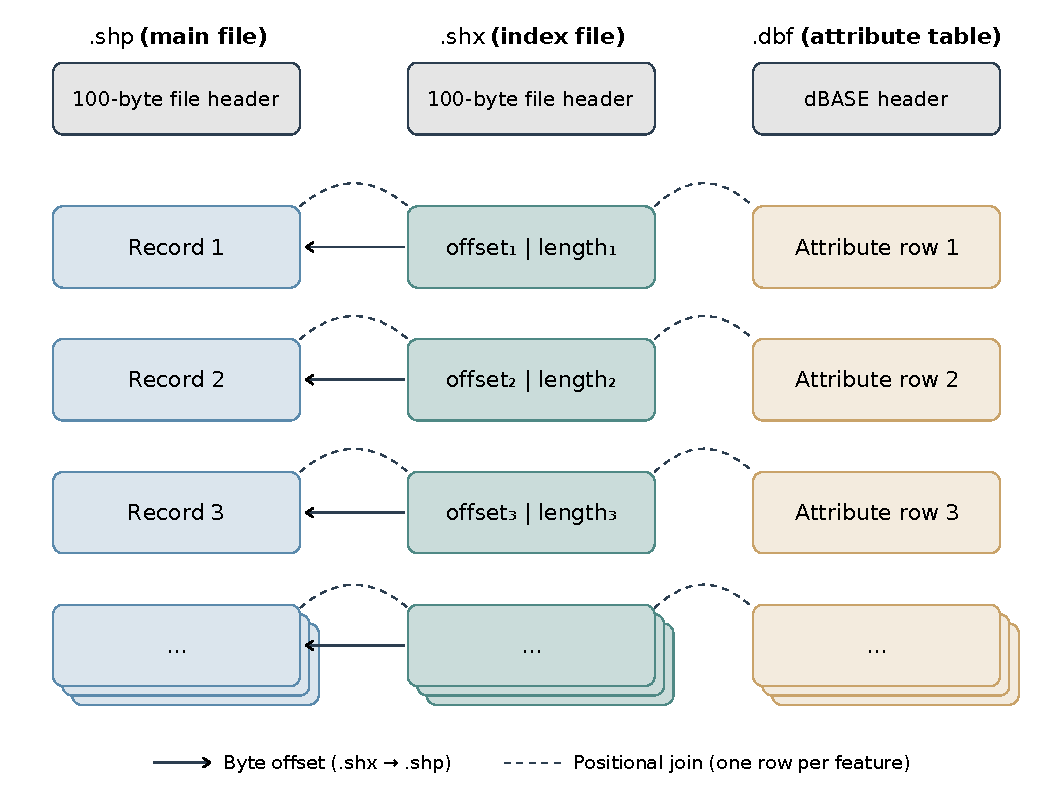
\includegraphics[width=0.7\textwidth]{Chapters/02-background/sub-chapters/figures/02-shapefile-linkage.pdf}
    \caption[Component-file linkage in a Shapefile]{Component-file linkage in a Shapefile. Each entry in the \texttt{.shx} index points (solid arrow) to the byte offset of the corresponding variable-length record in the \texttt{.shp} main file. The \texttt{.dbf} attribute table holds one row per feature in the same order as the \texttt{.shp} records, so attributes and geometries are joined by record position rather than by a key column (dashed connectors). Adapted from \textcite{esri1998_shapefile_technical_description}.}
    \label{fig:shapefile-linkage}
\end{figure}

A Shapefile is restricted to a single geometry type per file, chosen from \num{14} values that include 2D, 3D, and measured variants of points, polylines, polygons, and multipoints \parencite{esri1998_shapefile_technical_description}. The format records no topology, the explicit characterization of spatial relationships and shared geometry between features \parencite{ogc2007_07036_gml_specification}. The original specification also defines no \acrshort{crs}, and this information is supplied instead through an auxiliary \acrshort{wkt} file that emerged as a de facto convention with later \acrshort{esri} products \parencite{esri1998_shapefile_technical_description, gdal2025_shapefile_driver}.

The \texttt{.shx} index provides direct access to any feature record by byte offset, but it is a record index rather than a spatial index, and cannot accelerate bounding-box or intersection queries. A spatial index must be created separately and stored in one of the auxiliary files in Table~\ref{tab:shapefile-components}, either \acrshort{esri}'s undocumented \texttt{.sbn}/\texttt{.sbx} files or the quadtree \texttt{.qix} files used by MapServer and \acrfull{gdal} \parencite{gdal2025_shapefile_driver}. Without such an index, evaluating a spatial predicate requires a sequential scan of the \texttt{.shp} file, reading and parsing every record in order, since the format carries no per-record or per-block metadata that would let a reader skip features without first reading them.

% Academic rewrite
The format also imposes constraints on file size and value representation. The \texttt{.shp} file addresses its records through \num{32}-bit offsets counted in \num{16}-bit words \parencite{esri1998_shapefile_technical_description}, so the format itself tops out near \num{8}~GB, with the \acrshort{gdal} implementation capping it lower at \num{4}~GB \parencite{gdal2025_shapefile_driver}. In practice a \num{2}~GB size limit applies to each component file for compatibility across software \parencite{esri2024_arcmap_shapefile_output}, so datasets exceeding this size must be partitioned across multiple Shapefiles. Floating-point values are stored as text rather than binary, which can introduce rounding errors on read and write \parencite{esri2024_arcmap_shapefile_output}, and the format has no native representation of \texttt{null}: \acrshort{esri} software writes null values as zero \parencite{esri2024_arcmap_shapefile_output}.

\subsubsection{GeoJSON}
\label{background:spatial-data-formats-and-storage-models:file-formats:geojson}
GeoJSON is a text-based format for geographic data based on \acrfull{json}. The \acrfull{ietf} standardized it as \acrfull{rfc}~7946 in August 2016, replacing a 2008 community specification \parencite{butler2016_rfc7946_geojson_format}. Its \acrfull{iana} media type\footnote{A media type is a standardized label for the format of a resource, registered with \acrshort{iana}, that allows software to recognize how the content should be processed.} is \texttt{application/geo+json}, with file extensions \texttt{.json} or \texttt{.geojson} \parencite{butler2016_rfc7946_geojson_format}.

A GeoJSON document is a single \acrshort{json} object whose type is one of the seven \acrshort{ogc} Simple Features geometry types or one of two wrappers unique to GeoJSON. A \texttt{Feature} pairs a geometry with a \texttt{properties} object holding its attributes, and a \texttt{FeatureCollection} is a list of features. Unlike Shapefile's \texttt{.shp}/\texttt{.dbf} pairing, geometries and attributes are stored together and parsed as a single unit \parencite{butler2016_rfc7946_geojson_format}.

Coordinates are \acrshort{json} arrays of two or three numbers: longitude, latitude, and optional altitude. Implementations should not use more than three elements \parencite{butler2016_rfc7946_geojson_format}. \acrshort{rfc}~7946 requires all coordinates to be in WGS84 longitude and latitude (\texttt{OGC:CRS84}), removing support for alternative reference systems that caused interoperability problems \parencite{butler2016_rfc7946_geojson_format}. The standard also mandates the right-hand rule for polygon rings, a winding convention in which exterior rings run counterclockwise and holes clockwise to identify each ring's interior. For bounding boxes it uses \texttt{[west, south, east, north]} rather than \texttt{minx, miny, maxx, maxy} \parencite{butler2016_rfc7946_geojson_format}.

GeoJSON has no indexing mechanism. Unlike Shapefile's \texttt{.shx}, it lacks structures for fast access, row-group statistics, or embedded metadata identifying byte ranges. Any query, spatial or attribute-based, therefore requires parsing every Feature from the start of the file, because a \acrshort{json} parser cannot skip Features and must tokenize the entire document, scanning each character to recognize the structural delimiters that mark Feature boundaries. The \texttt{type} field may appear only after a long \texttt{features} array, so large files must be read in full before their structure can be confirmed \parencite{butler2016_rfc7946_geojson_format}.

GeoJSON is plain text and readable by any tool that supports \acrshort{json}, which has made it popular for web maps, \acrshort{json}-based \acrshort{api}s, and ad hoc data exchange. At scale, these same properties become limitations. Files cannot be partially parsed, which forces the entire document to be downloaded before use and makes the format unsuitable for cloud-optimized access \parencite{cngfoundation2024_cloud_optimized_geospatial_formats_guide}.

\subsubsection{Geography Markup Language}
\label{background:spatial-data-formats-and-storage-models:file-formats:geography-markup-language}
\acrfull{gml} is an \acrfull{xml}-based format for geographic information, standardized as \acrshort{ogc} 07-036 and \acrfull{iso} 19136:2007 \parencite{ogc2007_07036_gml_specification}. A \acrshort{gml} dataset is defined by a schema together with an instance document, which makes it less self-contained than GeoJSON or Shapefile \parencite{ogc2007_07036_gml_specification}. Its geometry model extends beyond Simple Features to non-linear curves, solids, and topology primitives \parencite{ogc2007_07036_gml_specification}. The format defines no native index \parencite{lu2005_advances_in_gml_geospatial_applications} and uses a verbose, text-based encoding \parencite{guo2010_effective_gml_documents_compressor}, so large datasets are impractical to query in place and are typically loaded into a spatial database for analysis \parencite{li2004_gml_storage_spatial_database}. \acrshort{gml} remains the default encoding for most data specifications under the European \acrfull{inspire} framework \parencite{ec2010_commission_regulation_1089_inspire, inspire2023_d27_encoding_guidelines}.

\subsubsection{GeoParquet}
\label{background:spatial-data-formats-and-storage-models:file-formats:geoparquet}
GeoParquet stores geospatial data in Apache Parquet, a widely adopted columnar file format for analytical workloads \parencite{ogc2024_geoparquet_specification_v110, lamb2022_querying_parquet_millisecond_latency}. Its cloud-native properties follow from Parquet itself, not from any geospatial extension, and reflect the broader shift from row-oriented to columnar storage in modern data platforms.

GeoParquet files follow Parquet's internal structure, illustrated in Figure~\ref{fig:geoparquet-file-format}. Rows are organized into row groups, contiguous and independently readable partitions, and within each group every column is stored separately so that a query touches only the columns it needs. The file footer holds a metadata index with the location and min/max statistics of every column in every row group \parencite{lamb2022_querying_parquet_millisecond_latency}. Geometries occupy a binary column encoded either in \acrshort{wkb} or in GeoArrow, a columnar alternative to WKB, so per-group statistics extend to geometry as well \parencite{ogc2024_geoparquet_specification_v110}.

\begin{figure}[H]
    \centering
    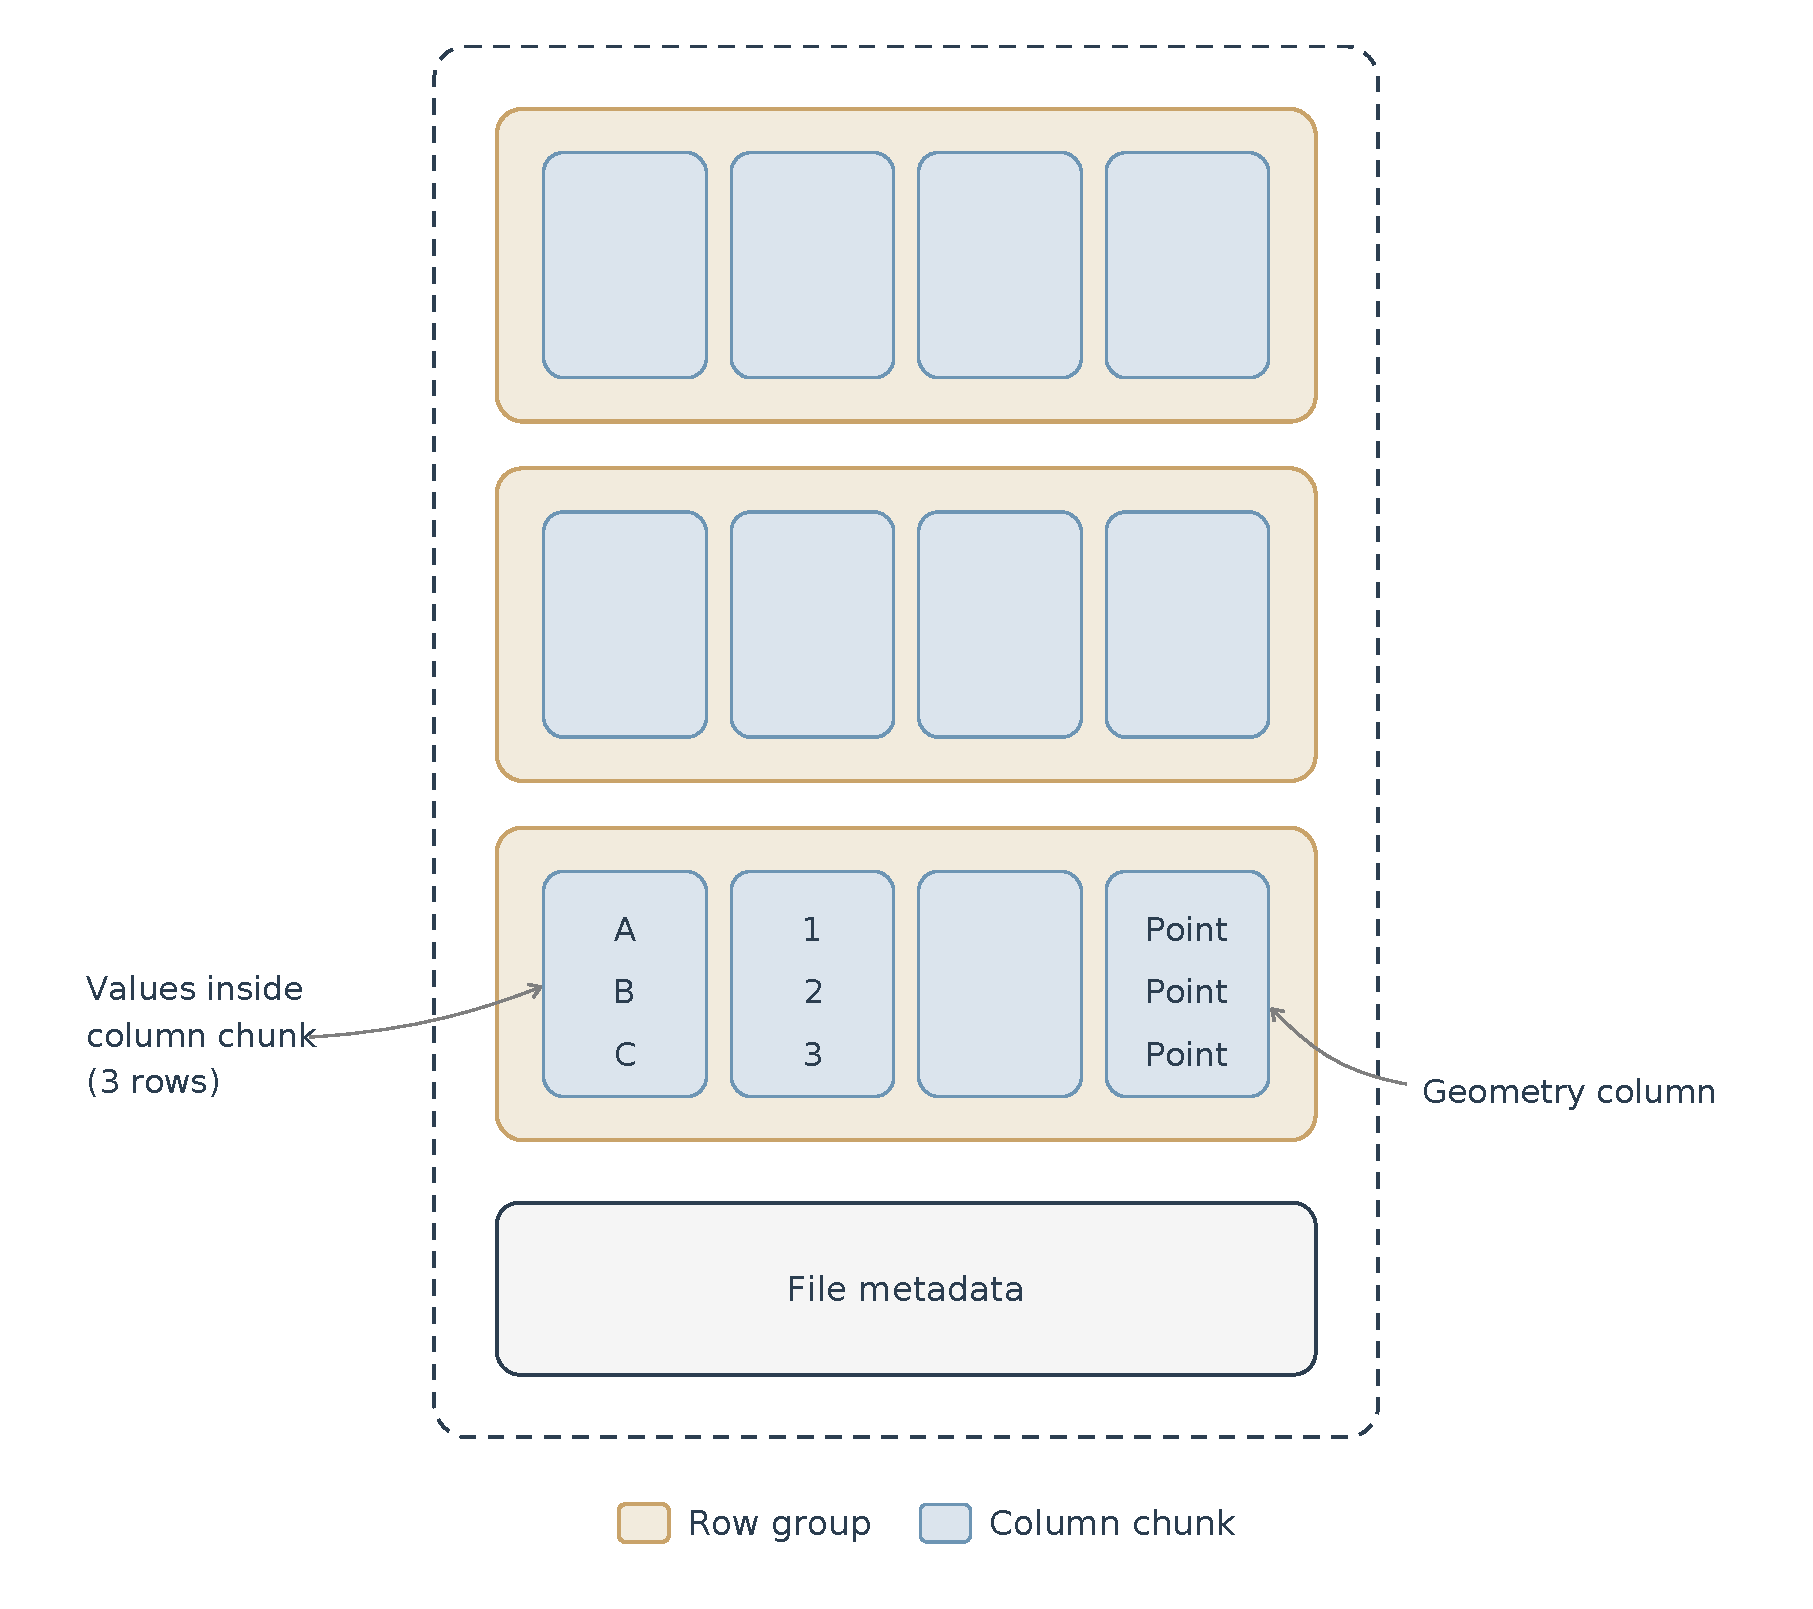
\includegraphics[width=0.75\textwidth]{Chapters/02-background/sub-chapters/figures/02-geoparquet-file-format.pdf}
    \caption[Internal structure of a GeoParquet file]{Internal structure of a GeoParquet file. Rows are grouped into row groups, each holding one column chunk per column, and the file footer holds the metadata index with location and min/max statistics for every column chunk. Adapted from \textcite{cngfoundation2024_geoparquet_guide}.}
    \label{fig:geoparquet-file-format}
\end{figure}

Coordinate reference systems are described in PROJJSON, a \acrshort{json} encoding of WKT2:2019, with \texttt{OGC:CRS84} (WGS84 longitude and latitude) as the default when none is specified \parencite{ogc2024_geoparquet_specification_v110}. The specification also fixes axis order to \texttt{(x, y)} regardless of the \acrshort{crs}, avoiding the latitude/longitude ambiguity that affects \acrshort{gml} \parencite{ogc2024_geoparquet_specification_v110}.

The format is built for selective reads. By comparing query predicates against each row group's min/max statistics in the footer, a reader can skip groups whose values cannot satisfy the predicate, an optimization known as predicate pushdown \parencite{lamb2022_querying_parquet_millisecond_latency}. The columnar layout further enables projection pushdown, so a reader fetches only the columns the query references \parencite{lamb2022_querying_parquet_millisecond_latency}. GeoParquet 1.1 extends this pruning to spatial predicates through an optional per-row bounding-box encoding with \texttt{xmin}, \texttt{ymin}, \texttt{xmax}, \texttt{ymax} columns, so spatial filters benefit from the same row-group skipping as scalar filters \parencite{ogc2024_geoparquet_specification_v110}. Although Parquet was designed for \acrfull{hdfs}, its access pattern transfers to commodity object storage because the two share similar performance characteristics \parencite{lamb2022_querying_parquet_millisecond_latency}. Readers therefore issue \acrshort{http} range requests for the footer and the row groups they need, leaving the rest of the file untransferred \parencite{cngfoundation2024_cloud_optimized_geospatial_formats_guide}.

The limitations follow from the same static columnar design. Parquet files are immutable, so any update or append requires rewriting the file in full \parencite{microsoft2024_direct_lake_parquet_immutability}. Workloads dominated by many small files also suffer, because each open incurs a separate footer fetch \parencite{cngfoundation2024_geoparquet_guide}. The format defines no spatial index proper; the 1.1 bounding-box covering enables row-group pruning but cannot stand in for an R-tree on complex joins or nearest-neighbor searches \parencite{cngfoundation2024_geoparquet_guide}. The geometry model is also narrower than some alternatives, omitting M values and non-linear geometry types and requiring geometry to sit as a top-level column rather than a nested field \parencite{ogc2024_geoparquet_specification_v110}. For best results, the specification recommends row groups of \numrange{50000}{150000} rows, spatial partitioning of files larger than \num{2}~GB, and compression with zstd, a general-purpose codec that balances speed and ratio \parencite{ogc2024_distributing_geoparquet}.

\subsection{File databases}
\label{background:spatial-data-formats-and-storage-models:file-databases}
A file database is a single, portable file that bundles the data, an embedded query engine, and indexes. Unlike a flat file, it answers queries using its own indexes. Unlike a server-based engine, in which a long-running server process accepts client queries and arbitrates concurrent access, a file database needs no such process. The engine is linked into the calling application as a library and reads the file through ordinary function calls, so file databases are easy to deploy and move between machines. The trade-off is write concurrency, the ability for multiple writers to modify the data simultaneously. With no server to arbitrate access, the database falls back on file-level coordination through operating-system file locks, which limits how many writers can operate at once. File databases therefore serve single-user analysis and data exchange well, but not workloads with many concurrent writes.

SpatiaLite and \acrshort{ogc} GeoPackage both build on SQLite, a public-domain, in-process \acrfull{sql} engine whose database is a single cross-platform file \parencite{sqlite2024_about, gaia2011_spatialite_manual, ogc2024_geopackage_encoding_standard_140}. Both store geometries in BLOB columns and index them with SQLite's R*Tree module \parencite{gaia2011_blob_geometry, sqlite2024_rtree_module, ogc2024_geopackage_encoding_standard_140}. The \acrshort{esri} \acrfull{fgdb} instead packages each table as binary files in a \texttt{.gdb} folder and indexes geometry with a proprietary grid-based structure whose layout is known publicly only through reverse engineering \parencite{rouault2013_filegdb_format_specification, gdal2025_openfilegdb_driver}. All three embed the engine in the file and coordinate access through file-level locks, so they share SQLite's single-writer constraint and are unsuited to network file systems or high-concurrency writes \parencite{sqlite2024_appropriate_uses}. None supports selective reads from object storage over \acrshort{http}, the property that defines the cloud-native tier, so no file-database configuration enters the benchmark.

\subsection{Full database engines}
\label{background:spatial-data-formats-and-storage-models:full-database-engines}
A full database engine stores spatial data in tables managed by a query engine that supports a query language, typically SQL, and treats concurrency, transactions, and indexing as first-class concerns, meaning the engine implements them directly rather than leaving them to the application. Two architectural patterns dominate. In the client/server model, exemplified by PostgreSQL, a long-running server process manages the database files and accepts connections from client applications. For each connection the server forks a new backend process, a separate operating-system process spawned on demand to serve that client, so that many clients can read and write concurrently \parencite{postgresql2024_architectural_fundamentals}. Concurrent access is coordinated through \acrfull{mvcc}, which gives each statement a consistent snapshot of the data without blocking readers behind writers \parencite{postgresql2024_concurrency_control}. In the in-process model, exemplified by DuckDB, the engine is a library linked into the calling application; there is no separate server process, and queries run in the application's own address space, the memory region the operating system allocates to a single running process \parencite{raasveldt2019_duckdb_embeddable_analytical_database}. The two models couple the query engine to the data alike, but make different trade-offs around concurrency, deployment, and the path between storage and compute. The two systems described next realize these patterns.

\subsubsection{PostGIS}
\label{background:spatial-data-formats-and-storage-models:full-database-engines:postgis}
PostGIS is an open-source extension for PostgreSQL that adds spatial types, functions, and indexes \parencite{postgis2024_manual_34}. An extension here is a loadable module that PostgreSQL registers through its own catalog, so installed extensions behave as native parts of the database. The user enables it with \texttt{CREATE EXTENSION postgis}, and optional companion extensions add raster, topology, and SFCGAL-based 3D operations \parencite{postgis2024_manual_34}. Because PostGIS sits inside PostgreSQL, it inherits the database's transactional machinery: \acrshort{mvcc} concurrency control, which gives every statement a consistent snapshot of the data so readers never block writers \parencite{postgresql2024_concurrency_control}, \acrshort{wal}-based crash recovery \parencite{postgresql2024_wal}, and \acrfull{rbac} \parencite{postgresql2024_roles}. The extension reads and writes a broad set of formats, including \acrshort{wkt}, \acrshort{wkb}, \acrshort{ewkt}, \acrshort{ewkb}, GeoJSON, \acrshort{gml}, \acrfull{kml}, and \acrfull{svg}, which keeps it interoperable with most geospatial tools \parencite{postgis2024_manual_34}.

Unlike the formats discussed earlier in this chapter, PostGIS defines no file layout of its own. Spatial data resides in ordinary PostgreSQL tables \parencite{postgis2024_manual_34} and is managed by a long-running server process \parencite{postgresql2024_architectural_fundamentals}. To comply with the \acrshort{ogc} Simple Features for \acrshort{sql} specification, the extension maintains two metadata tables: \texttt{spatial\_ref\_sys}, which registers coordinate reference systems, and \texttt{geometry\_columns}, which records each spatial table's geometry column \parencite{postgis2024_manual_34}.

PostGIS exposes two spatial types built on different geometric models. The core \texttt{GEOMETRY} type stores planar geometry in any coordinate system identified by SRID and supports the full \acrshort{ogc} Simple Features geometry set, including M, Z, and ZM variants \parencite{postgis2024_manual_34}. The \texttt{GEOGRAPHY} type targets geodetic computation: it accepts any longitude/latitude-based \acrshort{srs}, returns measurements in meters, and covers a smaller geometry set that excludes curves, \acrlong{tin}s (\acrshort{tin}), and polyhedral surfaces \parencite{postgis2024_manual_34}. A large library of geometry-processing functions complements these types, with further capability added through the raster, topology, and SFCGAL extensions \parencite{postgis2024_manual_34}.

Spatial indexing in PostGIS builds on PostgreSQL's \acrshort{gist} framework, with an R-tree as the default spatial access method \parencite{postgis2024_manual_34, hellerstein1995_generalized_search_trees_database_systems}. \acrshort{gist} is an extensible structure that hosts B+-trees, R-trees, and other tree-based indexes behind a common set of operations \parencite{hellerstein1995_generalized_search_trees_database_systems}. PostGIS also supports \acrfull{spgist} indexes for quadtrees and k-d trees, and \acrfull{brin} indexes, which store per-block summary statistics rather than per-row entries and suit read-mostly data \parencite{postgis2024_manual_34}. Only bounding-box-based operators use the spatial index directly; functions such as \texttt{ST\_Distance} benefit from the index only when a bounding-box predicate is also supplied \parencite{postgis2024_manual_34}.

PostGIS's main limitation for cloud deployments is architectural rather than one of scale. Storage and compute are tightly coupled in the PostgreSQL model \parencite{dageville2016_snowflake_elastic_data_warehouse}: all data must be loaded into the server, and every query executes inside the server process \parencite{postgresql2024_architectural_fundamentals}, which makes PostGIS a poor fit for workflows that read directly from object storage \parencite{pang2024_storage_disaggregated_databases}. Client connections are likewise mediated by the server \parencite{postgresql2024_architectural_fundamentals}. Scaling out across machines therefore requires either replication, copying the data to additional servers, or sharding, partitioning the data across servers so each holds a subset \parencite{stonebraker1986_case_for_shared_nothing}. Cloud-native file formats, by contrast, let many compute processes read the same file directly from object storage without routing through a central server.

\subsubsection{DuckDB with the spatial extension}
\label{background:spatial-data-formats-and-storage-models:full-database-engines:duckdb-with-the-spatial-extension}
DuckDB is an in-process database management system for analytical workloads, much as SQLite serves transactional workloads dominated by small individual reads and writes \parencite{raasveldt2019_duckdb_embeddable_analytical_database}. Applications embed the engine and run queries in their own process, with no separate server required \parencite{raasveldt2019_duckdb_embeddable_analytical_database}. Its \acrshort{sql} dialect resembles PostgreSQL \parencite{duckdb2025_sql_introduction}. Spatial support is added by the \texttt{spatial} extension, which provides a \texttt{GEOMETRY} type based on the \acrshort{ogc} Simple Features model and integrates GEOS, \acrshort{gdal}, and PROJ for algorithms, format conversion, and coordinate transformation \parencite{gabrielsson2023_postgeese_duckdb_spatial_extension, duckdb2025_spatial_extension_overview}.

Like PostGIS, DuckDB does not define a file layout for spatial data. Tables loaded into DuckDB, known as managed tables, sit in the engine's own internal storage format, which partitions them into compressed column blocks and tracks per-block minimum and maximum statistics so that irrelevant blocks are skipped at query time \parencite{raasveldt2019_duckdb_embeddable_analytical_database}. Execution is vectorized: rather than processing one row at a time, query operators such as scans, filters, joins, and aggregations operate on fixed-size column-oriented containers called Vectors \parencite{duckdb2025_vector}. DuckDB can also operate directly on external files. The \texttt{httpfs} extension enables reading Parquet and other supported formats from \acrshort{http}, S3, Google Cloud Storage, and similar object storage \parencite{duckdb2025_documentation_httpfs}. Through \acrshort{gdal}, the spatial extension supports over \num{50} vector formats via the \texttt{ST\_Read} table function, so formats such as Shapefile, GeoPackage, or GeoJSON can be queried directly with \acrshort{sql} without explicit import \parencite{gabrielsson2023_postgeese_duckdb_spatial_extension}.

The core spatial type is \texttt{GEOMETRY}, based on the \acrshort{ogc} Simple Features model, and a large library of \texttt{ST\_}-prefixed functions handles geometry processing, format conversion, and coordinate transformation \parencite{gabrielsson2023_postgeese_duckdb_spatial_extension, duckdb2025_spatial_extension_overview}. From version 1.5, \texttt{GEOMETRY} became a built-in DuckDB type, though its functions remain in the spatial extension \parencite{duckdb2025_spatial_extension_overview}. The extension also includes experimental columnar native types such as \texttt{POINT\_2D} and \texttt{POLYGON\_2D}, which trade flexibility for better compression and faster execution \parencite{gabrielsson2023_postgeese_duckdb_spatial_extension, duckdb2025_spatial_extension_overview}.

{\sloppy
Spatial indexing in DuckDB uses an R-tree whose leaf nodes store the approximate minimum bounding rectangle of each geometry. The index is consulted when the query filter includes intersection-implying predicates such as \texttt{ST\_Intersects}, \texttt{ST\_Within}, or \texttt{ST\_Contains} \parencite{duckdb2025_spatial_extension_rtree_indexes}. DuckDB also keeps automatic min/max indexes for general-purpose data types, which act as zonemaps for predicate pruning \parencite{duckdb2025_documentation_indexes}. For Parquet files, DuckDB supports both projection and predicate pushdown to remote sources, reading only the required columns and skipping row groups that do not match the filter \parencite{duckdb2025_parquet_overview, duckdb2025_documentation_httpfs}.
\par}

DuckDB combines an in-process query engine, a Simple Features geometry type, and direct access to object storage, placing it between traditional and cloud-native systems. It offers a \acrshort{sql} interface and transactional behavior but can also operate on cloud-native files in object storage without loading them into managed tables. DuckDB is a single-node engine and scales vertically by adding resources to one machine rather than horizontally by distributing work across nodes \parencite{duckdb2025_scalability_faq}. Workloads that exceed one machine cannot be handled by adding more DuckDB nodes. Current limitations of the spatial extension include no spherical geometry, no Z or M dimensions in \texttt{GEOMETRY}, and no support for curve or polyhedral-surface types \parencite{gabrielsson2023_postgeese_duckdb_spatial_extension, duckdb2025_spatial_extension_overview}.

The two database engines compared above share a common foundation: a \acrshort{sql} query engine, an \acrshort{ogc} Simple Features geometry type, and R-tree spatial indexing. They differ in architecture. PostGIS runs as a server-based extension to PostgreSQL and scales vertically or through replication and sharding. DuckDB is an in-process single-node engine that can also read cloud-native files in object storage directly.

\subsection{In-memory dataframe libraries}
\label{background:spatial-data-formats-and-storage-models:in-memory-dataframe-libraries}

A fourth model reads spatial data into program memory and operates on it there, with no embedded query engine and no separate server process. In the Python ecosystem its established representative is GeoPandas \parencite{jordahl2024_geopandas}, which extends the pandas dataframe \parencite{mckinney2010_data_structures_statistical_computing} with a geometry column. A table of features then becomes a \texttt{GeoDataFrame} held entirely in the address space of the calling process, and analysis proceeds by calling library functions on that object rather than by issuing queries to an engine. Geometry operations are delegated to Shapely, the default backend since GeoPandas 0.14, which exposes the GEOS geometry library \parencite{geopandas2024_pygeos_to_shapely}. Fiona or pyogrio handle file \acrshort{io} over \acrshort{gdal}, and pyproj handles coordinate transformation over PROJ \parencite{jordahl2024_geopandas}.

Like the database engines, GeoPandas defines no on-disk format of its own. It reads and writes through the \acrshort{gdal} driver stack, and through the pyarrow library for GeoParquet and Feather, the columnar formats built on Apache Arrow \parencite{geopandas2024_reading_and_writing_files}. By default, a read materializes an entire layer into memory as a \texttt{GeoDataFrame} \parencite{geopandas2024_reading_and_writing_files, geopandas2024_read_file}. The reader can narrow what is loaded by passing a bounding box or geometry mask, a row slice, a column subset, or an \acrshort{sql} attribute filter, each delegated to the \acrshort{gdal} engine, but these filters are opt-in \parencite{geopandas2024_reading_and_writing_files, geopandas2024_read_file}. Shapely 2.0 vectorizes geometry operations, applying GEOS to the whole array of geometries at once rather than processing one geometry at a time in Python \parencite{geopandas2024_pygeos_to_shapely}.

GeoPandas keeps no persistent spatial index. On first access to the \texttt{.sindex} property, it builds an in-memory R-tree, the Sort-Tile-Recursive tree provided by Shapely, and caches it on the object \parencite{geopandas2024_spatial_indexing}. The spatial join, overlay, and clip operations consult this index automatically, whereas an elementwise predicate such as testing intersection against a single geometry does not, instead testing every geometry in turn \parencite{geopandas2024_spatial_indexing}.

Because the dataset occupies the memory of a single process, GeoPandas scales only vertically, by enlarging that machine, and the core library spills nothing to disk. The separate dask-geopandas project provides distributed or larger-than-memory execution \parencite{geopandas2024_dask_geopandas}. GeoPandas maintains no managed-table storage, no transactions, and no concurrency control. It therefore embodies the traditional read model, in which analysis begins by materializing the full dataset in memory \parencite{jordahl2024_geopandas}, in contrast to the selective, range-based reads the cloud-native formats support. This memory ceiling bounds the dataset size GeoPandas can process.

\subsection{Summary}
\label{background:spatial-data-formats-and-storage-models:summary}

% Academic rewrite
The formats and engines in this section fall into three architectural tiers: flat files, file databases, and full database engines. Table~\ref{tab:format-summary} compares them along three dimensions that shape benchmark outcomes --- native spatial indexing, primary access pattern, and support for cloud-native access through \acrshort{http} range requests on object storage --- with horizontal rules separating the tiers in the order introduced. Of these, four carry into the remainder of the thesis: Shapefile as the representative legacy flat file, read with the GeoPandas in-memory dataframe library described in Section~\ref{background:spatial-data-formats-and-storage-models:in-memory-dataframe-libraries}; GeoParquet as the cloud-native flat file; and two full database engines, the server-based PostGIS and the in-process DuckDB, whose cloud-native access is realised specifically when it reads GeoParquet over object storage --- the configuration used in the benchmark.

\begin{table}[H]
    \centering
    \footnotesize
    \setlength{\tabcolsep}{6pt}
    \renewcommand{\arraystretch}{1.2}
    \caption[Summary of spatial data formats and engines]{Spatial data formats and engines compared along the dimensions used in this thesis.}
    \label{tab:format-summary}
    \begin{tabularx}{\textwidth}{@{}l L L c@{}}
        \toprule
        \textbf{Format / engine} & \textbf{Native spatial index} & \textbf{Access pattern} & \textbf{Cloud-native} \\
        \midrule
        Shapefile         & Optional sidecar           & Sequential scan                       & No      \\
        GeoJSON           & None                       & Full parse                            & No      \\
        \acrshort{gml}    & None                       & Full parse                            & No      \\
        GeoParquet        & Optional bbox covering     & Range requests, pushdown              & Yes     \\
        \midrule
        SQLite/SpatiaLite & R*Tree                     & Engine through file                   & No      \\
        GeoPackage        & R*Tree                     & Engine through file                   & No      \\
        File Geodatabase  & Grid-based (proprietary)   & Engine through files                  & No      \\
        \midrule
        PostGIS           & R-tree on \acrshort{gist}  & Server-mediated \acrshort{sql}        & No      \\
        DuckDB + spatial  & R-tree                     & In-process \acrshort{sql} or remote   & Partial \\
        \bottomrule
    \end{tabularx}
\end{table}
% \section{Distributed spatial processing}
% \label{sec:distributed-spatial-processing}
% Section \ref{background:cloud-native-data-architecture:distributed-and-non-distributed-computation} introduced the trade-off between distributed and non-distributed compute, and Section \ref{background:spatial-data-formats-and-storage-models:full-database-engines} described PostGIS and DuckDB as full single-node engines. This section turns to the third architectural class compared in this thesis: distributed spatial processing on a cluster of executors that share neither memory nor local disk. The aim is to make precise where time and cost are spent when a spatial query runs on a Spark-based engine, so that observed differences against PostGIS and DuckDB can be attributed to specific mechanisms rather than to the label \enquote{distributed}. Section \ref{background:distributed-spatial-processing:the-lifecycle-of-a-distributed-spatial-query} traces a query through the engine and names the stages that account for wall-clock time. Section \ref{background:distributed-spatial-processing:spatial-partitioning-and-parallel-efficiency} identifies spatial partitioning as the lever that decides whether the lifecycle parallelizes. Section \ref{background:distributed-spatial-processing:distributed-spatial-operations} reviews the dominant operations on this lifecycle, and Sections \ref{background:distributed-spatial-processing:apache-sedona} and \ref{background:distributed-spatial-processing:databricks-as-a-sedona-run-time} describe the concrete implementations evaluated in this thesis.

\section{Distributed spatial processing}
\label{background:distributed-spatial-processing}
Section \ref{background:cloud-native-data-architecture:distributed-and-non-distributed-computation} introduced the trade-off between distributed and non-distributed compute, and Section \ref{background:spatial-data-formats-and-storage-models:full-database-engines} described PostGIS and DuckDB as full single-node engines. This section turns to the third architectural class compared in this thesis: distributed spatial processing on a shared-nothing cluster, in which executors share neither memory nor local disk. The aim is to specify where time and cost are spent when a spatial query runs on an engine built on Apache Spark, a general-purpose cluster-computing framework for in-memory distributed processing. Observed differences against PostGIS and DuckDB can then be attributed to specific mechanisms rather than to the label \enquote{distributed}. Section \ref{background:distributed-spatial-processing:the-lifecycle-of-a-distributed-spatial-query} traces a query through the engine and names the stages that account for wall-clock time, the elapsed time from query submission to result return. Section \ref{background:distributed-spatial-processing:spatial-partitioning-and-parallel-efficiency} identifies spatial partitioning as the lever that decides whether the lifecycle parallelizes. Section \ref{background:distributed-spatial-processing:distributed-spatial-operations} reviews the dominant operations on this lifecycle, and Sections \ref{background:distributed-spatial-processing:apache-sedona} and \ref{background:distributed-spatial-processing:databricks-as-a-sedona-run-time} describe the concrete implementations evaluated in this thesis.

% \subsection{The lifecycle of a distributed spatial query}
% \label{subsec:lifecycle}
% A query submitted to a Spark-based engine such as Apache Sedona is first planned on a single coordinator process, the \emph{driver}, which uses the Catalyst optimizer to translate the \acrshort{sql} or DataFrame input into a physical plan that the cluster will execute \parencite{armbrust2015_spark_sql_relational_data_processing, spark2024_cluster_mode_overview}. This planning phase runs sequentially before any task is dispatched, and on workloads with short execution times, it is part of the fixed overhead that does not shrink with additional workers.

% The physical plan executes against an underlying abstraction of partitioned, fault-tolerant collections. The \acrfull{rdd} is a \enquote{distributed memory abstraction that lets programmers perform in-memory computations on large clusters in a fault-tolerant manner} \parencite{zaharia2012_resilient_distributed_datasets}. DataFrames in Spark \acrshort{sql} compile down to \acrshort{rdd} operations after Catalyst's physical planning phase \parencite{armbrust2015_spark_sql_relational_data_processing}. The driver translates the physical plan into a \acrfull{dag} of \emph{stages}, each consisting of \emph{tasks} that run in parallel on \emph{executors}, the \acrshort{jvm} processes that hold cached partitions and execute task code \parencite{zaharia2012_resilient_distributed_datasets, spark2024_cluster_mode_overview}.

% Within a stage, transformations run locally on each executor \parencite{zaharia2012_resilient_distributed_datasets}. Operations that require records from many partitions trigger a \emph{shuffle}, which writes intermediate data to local disk and fetches it across the network in the next stage \parencite{zaharia2012_resilient_distributed_datasets, spark2024_job_scheduling}. Shuffles transfer data between executors and are a major source of network traffic during a query, and the volume of bytes they move, the \emph{shuffle volume}, affects both elapsed time and bytes received.

% Two phases of this lifecycle are worth naming. The \emph{executor read time} is the time spent reading input partitions from storage at the start of the query, and is dominated by network round-trips when the data lives in Azure object storage rather than on local disk. \emph{Driver collection} is the time spent at the end of the query returning results to the driver via an action such as \texttt{collect}, and is sequential in the size of the result set \parencite{zaharia2012_resilient_distributed_datasets}. Figure \ref{fig:distributed-spatial-query-lifecycle} situates both phases within the full lifecycle.

% \begin{figure}[H]
% 	\centering
% 	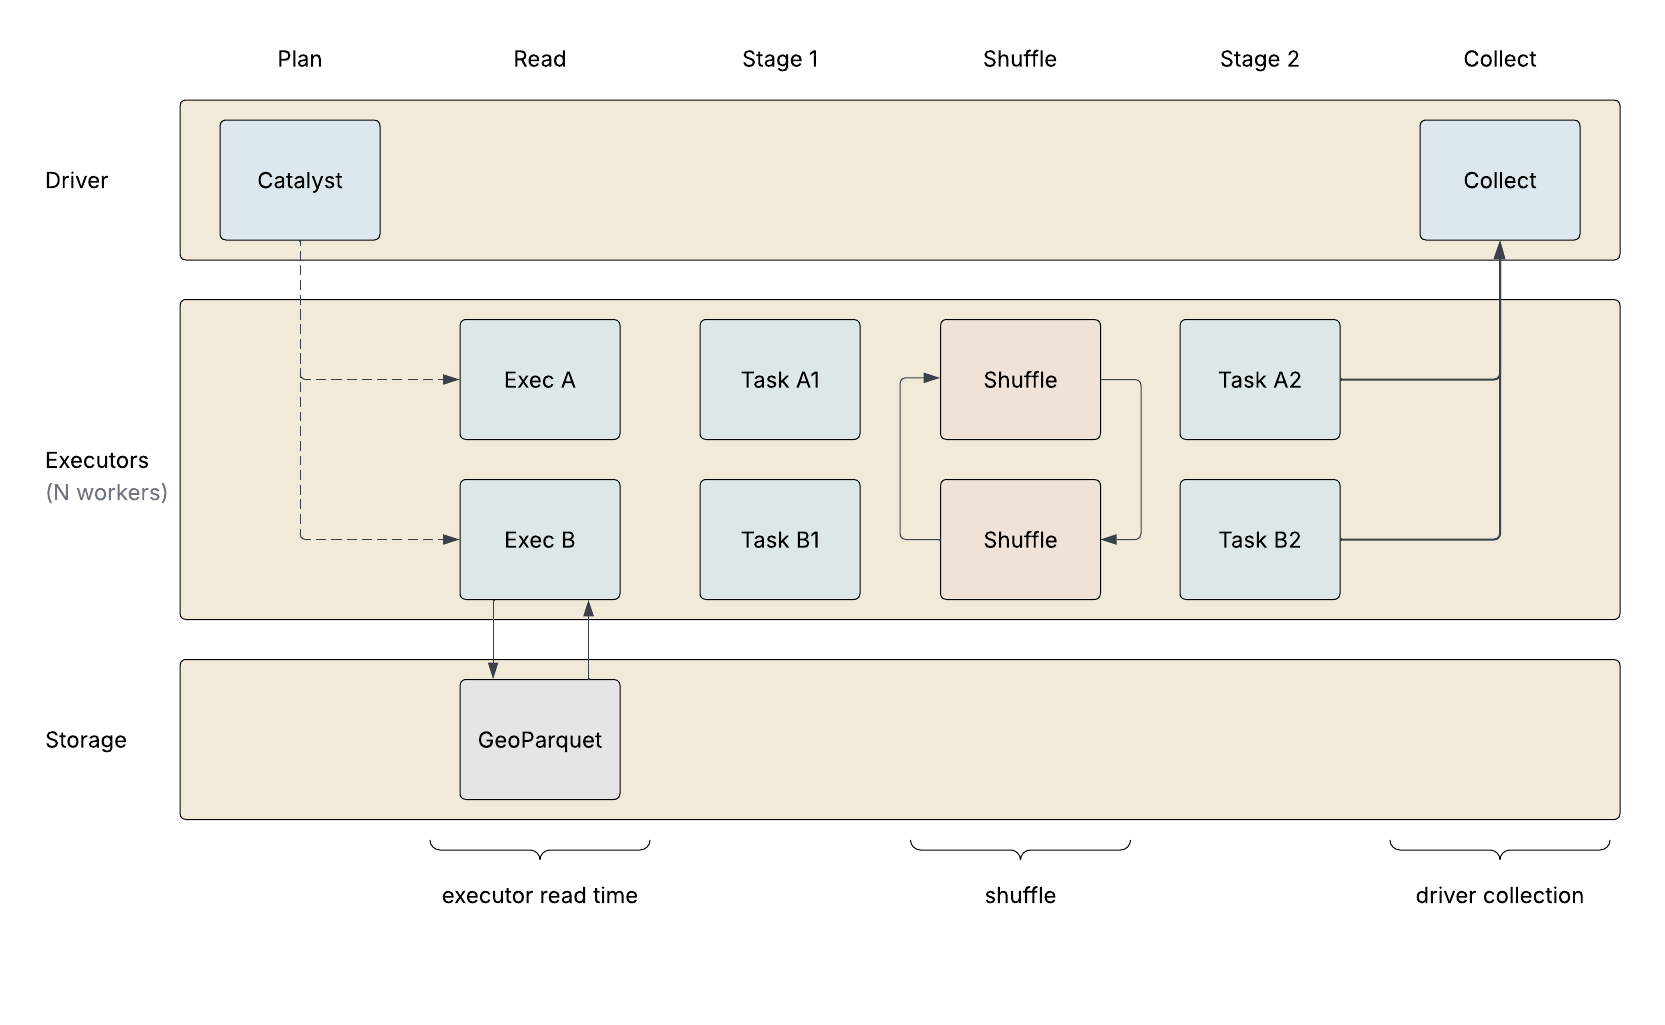
\includegraphics[width=0.8\textwidth]{Chapters/02-background/sub-chapters/figures/02-distributed-spatial-query-lifecycle.png}
% 	\caption[Lifecycle of a distributed spatial query]{Lifecycle of a distributed spatial query on a Spark-based engine, shown as a swimlane across the driver, executors, and object storage. The six columns trace the query from planning, through reading input partitions, two narrow stages separated by a shuffle, and final result collection. The brackets below the storage lane mark the three named phases referenced in the prose: \emph{executor read time}, \emph{shuffle}, and \emph{driver collection}. Inter-lane arrows distinguish the network channels. The dashed gray arrows from Catalyst to each executor carry the serialized plan and task descriptors at a small, input-independent cost. The arrows between the executors and storage carry the data reads, with volume scaling with input size. The coral arrows around the shuffle column carry intra-cluster traffic between executors as Stage~1 outputs are redistributed for Stage~2. The arrows from the Stage~2 tasks to Collect carry the result set back to the driver, with volume scaling with its size.}
%  	\label{fig:distributed-spatial-query-lifecycle}
% \end{figure}

% The lifecycle also determines how bytes are exchanged across the system, which the benchmark measures directly. Three channels carry the bulk of network traffic. The driver-to-executor channel carries the serialized plan and task descriptors, a small and largely fixed cost independent of input size \parencite{spark2024_cluster_mode_overview}. The executor-to-storage channel carries the actual data reads from object storage and scales with the input size and the number of files not pruned by metadata. The executor-to-driver channel at the end of the query carries either the full result set, when the query ends in an action that collects rows, or only a small aggregate such as a row count, when the query ends in a write or a count action \parencite{zaharia2012_resilient_distributed_datasets}. The total bytes transferred reported by the benchmark is the sum of these three channels, and the relative split among them is one of the signals available to attribute observed performance to specific parts of the lifecycle.

\subsection{The lifecycle of a distributed spatial query}
\label{background:distributed-spatial-processing:the-lifecycle-of-a-distributed-spatial-query}
A query submitted to a Spark-based engine such as Apache Sedona is first planned on a single coordinator process, the driver, which uses the Catalyst optimizer, Spark's query planner, to translate the \acrshort{sql} or DataFrame input into a physical plan, the concrete sequence of operations the cluster will execute \parencite{armbrust2015_spark_sql_relational_data_processing, spark2024_cluster_mode_overview}. A DataFrame is Spark's tabular abstraction over a distributed collection of rows, comparable in shape to a relational table \parencite{armbrust2015_spark_sql_relational_data_processing}. Planning runs sequentially before any task is dispatched, so on workloads with short execution times it constitutes fixed overhead that does not shrink with additional workers.

The physical plan executes against an underlying abstraction of partitioned, fault-tolerant collections. The \acrfull{rdd} is a \enquote{distributed memory abstraction that lets programmers perform in-memory computations on large clusters in a fault-tolerant manner} \parencite{zaharia2012_resilient_distributed_datasets}. DataFrames in Spark \acrshort{sql}, Spark's relational query module, compile down to \acrshort{rdd} operations after Catalyst's physical planning phase \parencite{armbrust2015_spark_sql_relational_data_processing}. The driver translates the physical plan into a \acrfull{dag} of \emph{stages}, each consisting of \emph{tasks} that run in parallel on \emph{executors}, the \acrfull{jvm} processes that hold cached partitions and execute task code \parencite{zaharia2012_resilient_distributed_datasets, spark2024_cluster_mode_overview}. The \acrshort{jvm} is the Java runtime that hosts Spark code on each worker.

Within a stage, transformations run locally on each executor, where a transformation is a lazy operation such as filter or map that describes a new dataset rather than producing one immediately \parencite{zaharia2012_resilient_distributed_datasets}. Operations that require records from many partitions trigger a \emph{shuffle}, which writes intermediate data to local disk and fetches it across the network in the next stage \parencite{zaharia2012_resilient_distributed_datasets, spark2024_job_scheduling}. Shuffles transfer data between executors and are a major source of network traffic during a query, and the volume of bytes they move, the \emph{shuffle volume}, affects both elapsed time and bytes received.

Two phases of this lifecycle are worth naming. The \emph{executor read time} is the time spent reading input partitions from storage at the start of the query, dominated by network round-trips when the data lives in Azure object storage rather than on local disk. \emph{Driver collection} is the time spent at the end of the query returning results to the driver via an action such as \texttt{collect}; an action is the operation that forces accumulated transformations to execute, and the phase itself is sequential in the size of the result set \parencite{zaharia2012_resilient_distributed_datasets}. Figure \ref{fig:distributed-spatial-query-lifecycle} situates both phases within the full lifecycle.

\begin{figure}[H]
	\centering
	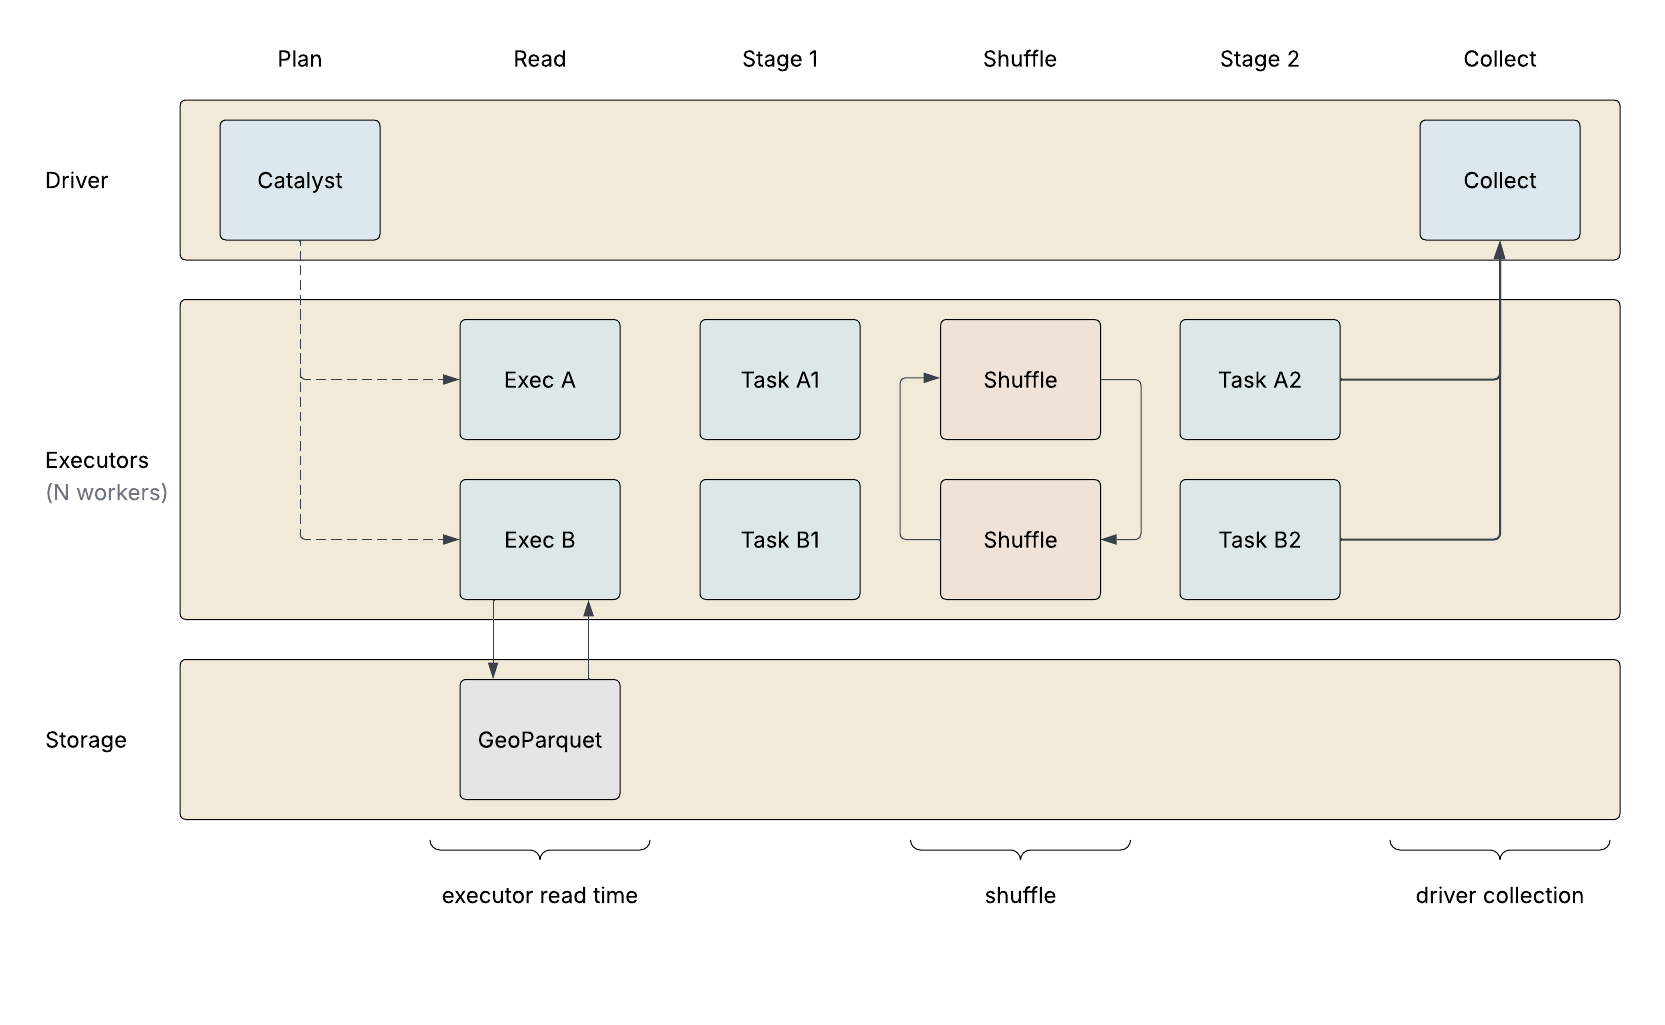
\includegraphics[width=0.8\textwidth]{Chapters/02-background/sub-chapters/figures/02-distributed-spatial-query-lifecycle.png}
	\caption[Lifecycle of a distributed spatial query]{Lifecycle of a distributed spatial query on a Spark-based engine, shown as a swimlane across the driver, executors, and object storage. The six columns trace the query from planning, through reading input partitions, two narrow stages separated by a shuffle, and final result collection. The brackets below the storage lane mark the three named phases referenced in the prose: \emph{executor read time}, \emph{shuffle}, and \emph{driver collection}. Inter-lane arrows distinguish the network channels. The dashed gray arrows from Catalyst to each executor carry the serialized plan and task descriptors at a small, input-independent cost. The arrows between the executors and storage carry the data reads, with volume scaling with input size. The coral arrows around the shuffle column carry intra-cluster traffic between executors as Stage~1 outputs are redistributed for Stage~2. The arrows from the Stage~2 tasks to Collect carry the result set back to the driver, with volume scaling with its size.}
 	\label{fig:distributed-spatial-query-lifecycle}
\end{figure}

The lifecycle also determines how bytes are exchanged across the system, which the benchmark measures directly. Three channels carry the bulk of network traffic. The driver-to-executor channel carries the serialized plan and task descriptors, a small and largely fixed cost independent of input size \parencite{spark2024_cluster_mode_overview}. The executor-to-storage channel carries the actual data reads from object storage and scales with the input size and the number of files not pruned by metadata. The executor-to-driver channel at the end of the query carries either the full result set, when the query ends in an action that collects rows, or only a small aggregate such as a row count, when the query ends in a write or a count action \parencite{zaharia2012_resilient_distributed_datasets}. The total bytes transferred reported by the benchmark is the sum of these three channels, and the relative split among them is one of the signals available for attributing observed performance to specific parts of the lifecycle.

% \subsection{Spatial partitioning and parallel efficiency}
% \label{subsec:partitioning}
% The lifecycle parallelizes only if the input is split into roughly equal pieces of work that executors can process independently. The mechanism that does this splitting is a \emph{partitioner}, a function that assigns each input record to one of several partitions, each of which becomes a unit of work for an executor \parencite{spark2024_partitioner_api, zaharia2012_resilient_distributed_datasets}. Spark's built-in partitioners, hash and range, distribute records by hashing or sorting their keys \parencite{spark2024_partitioner_api}. Neither method considers the geometry of the records. Two polygons that share a boundary will typically land on different partitions under a hash partitioner, and any operation whose semantics depend on geometry therefore has to either compare every record against every other or repartition the data spatially before it can run efficiently, the latter being the approach taken by spatial extensions to Spark \parencite{yu2019_geospark_perspective_beyond}. Figure \ref{fig:hash-vs-spatial-partitioning} contrasts the two on the same set of features.
% 
% \begin{figure}[H]
% 	\centering
% 	\subfloat[Hash partitioning.\label{fig:hash-partitioning}]{%
% 		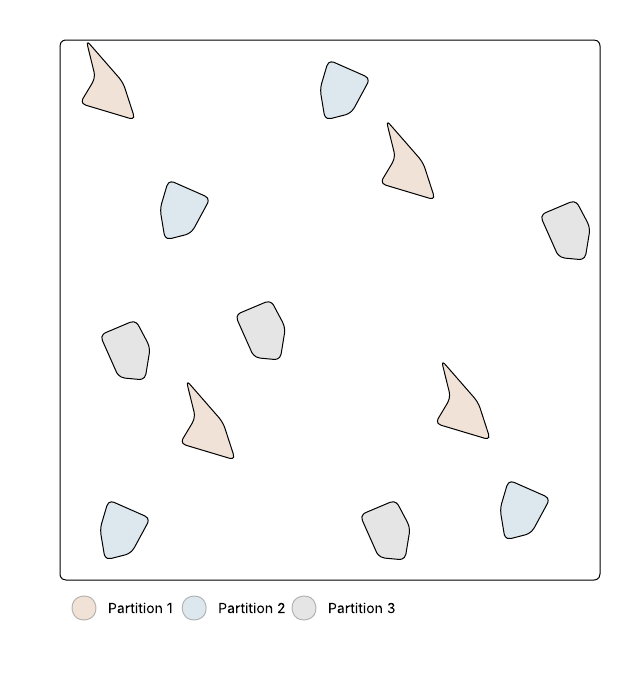
\includegraphics[valign=t, width=0.45\textwidth]{Chapters/02-background/sub-chapters/figures/02-hash-partitioning.png}%
% 	}
% 	\hfill
% 	\subfloat[Spatial partitioning.\label{fig:geographic-partitioning}]{%
% 		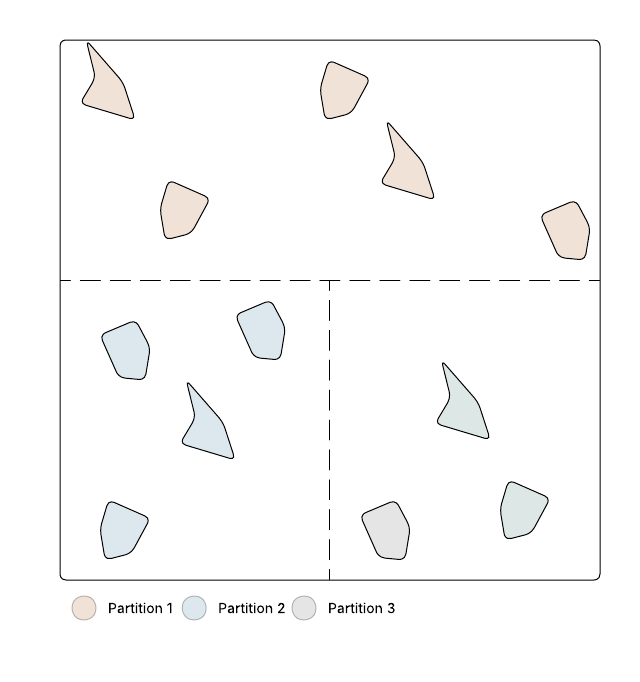
\includegraphics[valign=t, width=0.45\textwidth]{Chapters/02-background/sub-chapters/figures/02-geographic-partitioning.png}%
% 	}
% 	\caption[Hash versus spatial partitioning of the same features]{Hash versus spatial partitioning of the same set of features. Both panels show the same polygons in identical positions; color encodes partition assignment, with each color corresponding to one partition handled by a different executor. (a) Under hash partitioning, color is uncorrelated with position, so polygons that share a boundary in the plane typically land on different partitions. (b) Under spatial partitioning, the study area is divided into spatially contiguous cells (dashed dividers) and all polygons within a cell share a color, so locality in the plane is preserved as locality in partition assignment. Adapted from \parencite{eldawy2015_spatial_partitioning_techniques}.}
% 	\label{fig:hash-vs-spatial-partitioning}
% \end{figure}
% 
% Spatial partitioners replace this with a function of the geometry's location and extent. \textcite{yu2019_geospark_perspective_beyond} describes four such partitioners that have become standard in the Spark ecosystem: \enquote{uniform grid, R-tree, Quad-Tree, and KDB-Tree}. A uniform grid divides the study area into equal cells and is the cheapest to compute, but is sensitive to data density. The tree-based partitioners are constructed from a sample of the input so that each leaf cell contains a similar number of records, which yields more balanced partition sizes when the underlying distribution is skewed \parencite{yu2019_geospark_perspective_beyond}. After the global partitioner assigns records to partitions, each partition can build a local in-memory index, typically an R-tree or Quad-Tree, that accelerates per-partition processing \parencite{yu2019_geospark_perspective_beyond}. This two-tier design mirrors the partition-then-search structure of single-node spatial indexes such as the R-tree \parencite{guttman1984_rtree_dynamic_index}, applied here at the cluster scale.
% 
% Even with a spatial partitioner, work can still be distributed unevenly because the data, the query workload, or both are skewed. \textcite{tang2020_locationspark_distributed_spatial_query} term this failure mode \enquote{spatial query skew} and observe that traditional spatial partitioners balance data across cells but not the query load. The consequence they identify is that if many query windows fall inside one cell, the executor holding that cell becomes a straggler regardless of how evenly the records were distributed. The realized parallelism of the job is therefore bounded above by the most loaded partition: if a workload distributes evenly across $n$ executors, run-time falls roughly as $1/n$ until coordination cost dominates, but if a single partition holds half the join output, no number of additional executors will reduce run-time below the time taken to process that partition. Skew is a well-recognized cause of poor scaling in distributed query systems \parencite{kwon2012_skewtune_mitigating_skew}, and a likely explanation when a distributed engine fails to scale even though the work appears to decompose cleanly across executors.

\subsection{Spatial partitioning and parallel efficiency}
\label{background:distributed-spatial-processing:spatial-partitioning-and-parallel-efficiency}
The lifecycle parallelizes only when the input is split into pieces of roughly equal work that executors can process independently. This splitting is performed by a \emph{partitioner}, a function that assigns each input record to one of several partitions, each of which becomes a unit of work for an executor \parencite{spark2024_partitioner_api, zaharia2012_resilient_distributed_datasets}. Spark's built-in partitioners, hash and range, distribute records by hashing or sorting their keys, with no consideration of the geometry attached to each record \parencite{spark2024_partitioner_api}. Two polygons that share a boundary in the plane will typically land on different partitions under a hash partitioner, so any operation whose semantics depend on geometry must either compare every record against every other or repartition the data spatially before it can run efficiently. Spatial extensions to Spark take the latter route \parencite{yu2019_geospark_perspective_beyond}. Figure \ref{fig:hash-vs-spatial-partitioning} contrasts the two on the same set of features.

\begin{figure}[H]
	\centering
	\subfloat[Hash partitioning.\label{fig:hash-partitioning}]{%
		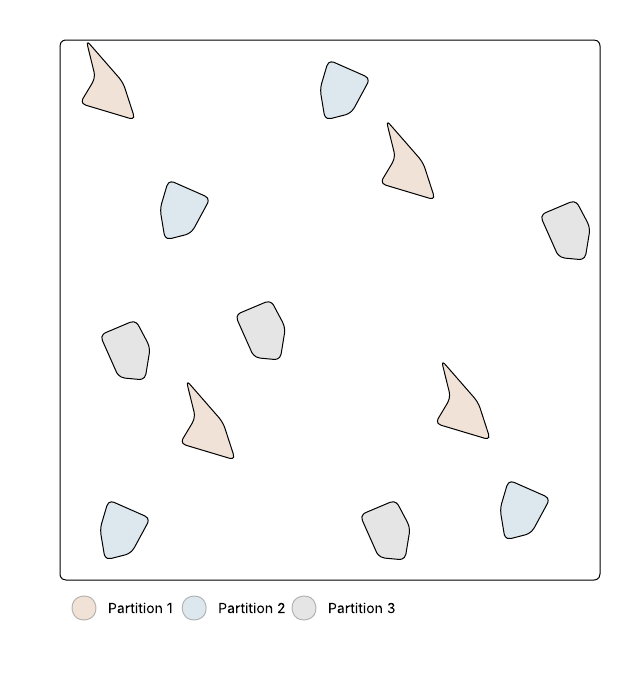
\includegraphics[valign=t, width=0.45\textwidth]{Chapters/02-background/sub-chapters/figures/02-hash-partitioning.png}%
	}
	\hfill
	\subfloat[Spatial partitioning.\label{fig:geographic-partitioning}]{%
		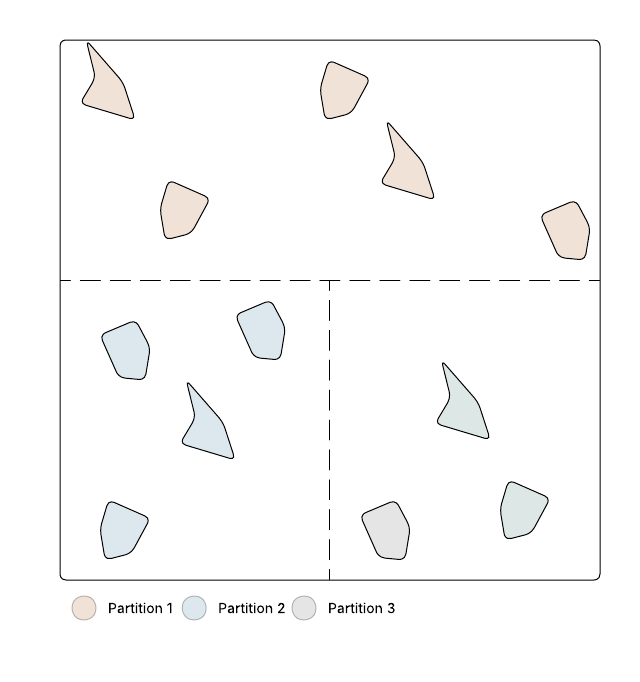
\includegraphics[valign=t, width=0.45\textwidth]{Chapters/02-background/sub-chapters/figures/02-geographic-partitioning.png}%
	}
	\caption[Hash versus spatial partitioning of the same features]{Hash versus spatial partitioning of the same set of features. Both panels show the same polygons in identical positions; color encodes partition assignment, with each color corresponding to one partition handled by a different executor. (a) Under hash partitioning, color is uncorrelated with position, so polygons that share a boundary in the plane typically land on different partitions. (b) Under spatial partitioning, the study area is divided into spatially contiguous cells (dashed dividers) and all polygons within a cell share a color, so locality in the plane is preserved as locality in partition assignment. Adapted from \parencite{eldawy2015_spatial_partitioning_techniques}.}
	\label{fig:hash-vs-spatial-partitioning}
\end{figure}

Spatial partitioners replace this key-based assignment with a function of each geometry's location and extent. \textcite{yu2019_geospark_perspective_beyond} describes four such partitioners that have become standard in the Spark ecosystem: \enquote{uniform grid, R-tree, Quad-Tree, and KDB-Tree}. A uniform grid divides the study area into equal cells and is the cheapest to compute, but it is sensitive to data density. The tree-based partitioners are constructed from a sample of the input so that each leaf cell contains a similar number of records, which yields more balanced partition sizes on skewed distributions \parencite{yu2019_geospark_perspective_beyond}. Once the global partitioner has assigned records to partitions, each partition can build a local in-memory index, typically an R-tree or Quad-Tree, that accelerates per-partition processing \parencite{yu2019_geospark_perspective_beyond}. This two-tier design mirrors the partition-then-search structure of single-node spatial indexes such as the R-tree \parencite{guttman1984_rtree_dynamic_index}, applied here at the cluster scale.

A spatial partitioner does not by itself guarantee even work distribution: the data, the query workload, or both may still be skewed. \textcite{tang2020_locationspark_distributed_spatial_query} term this failure mode \enquote{spatial query skew} and observe that traditional spatial partitioners balance data across cells but not query load. The consequence they identify is that when many query windows fall inside one cell, the executor holding that cell becomes a straggler, the single slow worker whose unfinished tasks hold up the rest of the stage, regardless of how evenly the records were distributed. The realized parallelism of the job, the speedup actually obtained as workers are added, is therefore bounded above by the most loaded partition: if a workload distributes evenly across $n$ executors, run-time falls roughly as $1/n$ until coordination cost dominates, but if a single partition holds half the join output, no number of additional executors will reduce run-time below the time taken to process that partition. Skew is a well-recognized cause of poor scaling in distributed query systems \parencite{kwon2012_skewtune_mitigating_skew}, and a likely explanation when a distributed engine fails to scale even though the work appears to decompose cleanly across executors.

% \subsection{Distributed spatial operations}
% \label{subsec:dist-operations}
% This subsection describes two spatial operations: the spatial range query, which filters one input against a fixed query window, and the spatial join, which evaluates a spatial predicate between two inputs. They differ sharply in how they exercise the lifecycle described in Section \ref{background:distributed-spatial-processing:the-lifecycle-of-a-distributed-spatial-query}.

% A spatial range query returns all geometries from an input that lie within a fixed query window \parencite{yu2019_geospark_perspective_beyond}. It runs entirely within a single stage: each partition filters its own contents independently without coordination with other executors \parencite{yu2019_geospark_perspective_beyond}. Any optimization that reduces the number of partitions scanned, therefore translates directly into run-time improvement. File-level bounding-box metadata in GeoParquet is one such optimization, as it allows the engine to skip files whose extent does not overlap the query window \parencite{sedona2024_geoparquet_loader}. A range query is the operation in which a distributed engine is hardest to distinguish from a single-node engine reading the same files, because the work naturally decomposes across files, regardless of the partitioner.

% The spatial join is the operation where the distribution either pays off or breaks down. A spatial join combines two inputs using a spatial predicate, such as intersection or distance, returning the records from each input that satisfy it \parencite{yu2019_geospark_perspective_beyond}. Because records from different executors must be brought together for comparison, the join is a wide operation that crosses a stage boundary \parencite{yu2019_geospark_perspective_beyond}, and two execution strategies have emerged to handle it. In a \emph{broadcast} join, the smaller input is shipped to every partition of the larger input, and each executor then performs a local join against its own partition \parencite{yu2019_geospark_perspective_beyond}. The strict shuffle cost is low, since no key-based redistribution is needed, though broadcasting the smaller input itself incurs network traffic that grows with its size. In a \emph{partitioned} join, both inputs are repartitioned by a common spatial partitioner so that records that could possibly satisfy the predicate land on the same executor; each executor then performs a local join within its own partition without further communication \parencite{yu2019_geospark_perspective_beyond}. Sedona supports KDB-Tree, Quad-Tree, and R-Tree partitioners for this strategy, with the requirement that both inputs be partitioned the same way \parencite{sedona2024_spatial_rdd_application}. Because a polygon may straddle partition boundaries, such records are duplicated into every overlapping partition to preserve correctness, and the system resolves the duplicates after the local join \parencite{yu2019_geospark_perspective_beyond}. The choice between broadcast and partitioned execution is a major lever on the run-time of a distributed spatial workload: a query that switches strategy at a size threshold will exhibit a discontinuous jump in runtime around that threshold. Figure \ref{fig:broadcast-vs-partitioned-join} contrasts the two strategies on the same pair of inputs.

% \begin{figure}[H]
% 	\centering
% 	\subfloat[Broadcast join.\label{fig:broadcast-join}]{%
% 		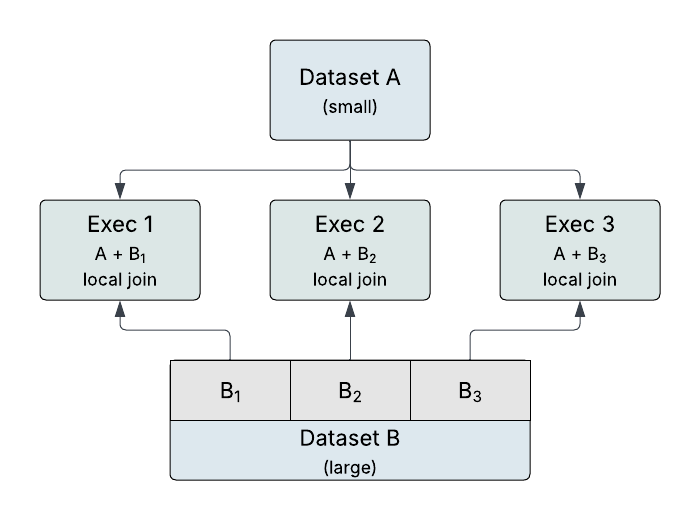
\includegraphics[valign=t, width=0.45\textwidth]{Chapters/02-background/sub-chapters/figures/02-broadcast-join.png}%
% 	}
% 	\hfill
% 	\subfloat[Partitioned join.\label{fig:partitioned-join}]{%
% 		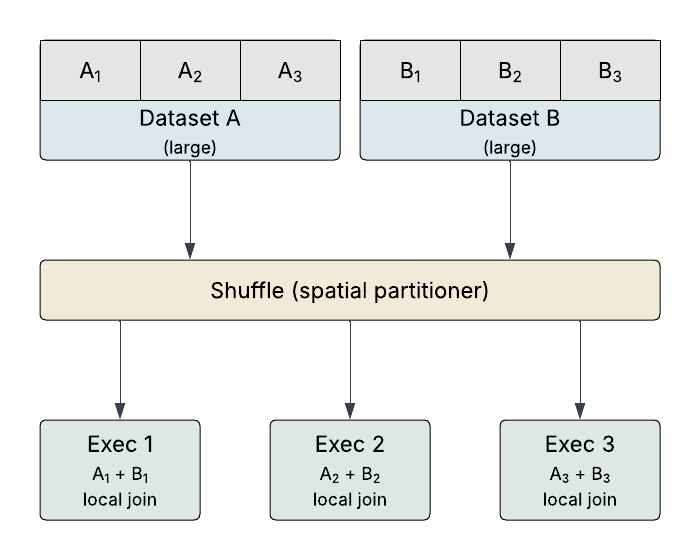
\includegraphics[valign=t, width=0.45\textwidth]{Chapters/02-background/sub-chapters/figures/02-partitioned-join.png}%
% 	}
% 	\caption[Broadcast versus partitioned spatial join]{Broadcast versus partitioned spatial join on the same two inputs. Both strategies converge on the same end state, three executors each performing a local join, but they differ sharply in where the network cost falls. (a) Broadcast: the small input A is shipped from a single source down to every executor; B's partitions are already resident on the executors and do not move, so network traffic scales only with the size of A. (b) Partitioned: both A and B flow through a shuffle that applies a common spatial partitioner, so spatially matching cells of A and B co-locate on each executor before the local join runs. Both inputs traverse the network in this case, and the heavy traffic is the cost of guaranteeing co-location.}
% 	\label{fig:broadcast-vs-partitioned-join}
% \end{figure}

\subsection{Distributed spatial operations}
\label{background:distributed-spatial-processing:distributed-spatial-operations}

Two spatial operations exercise the lifecycle of Section \ref{background:distributed-spatial-processing:the-lifecycle-of-a-distributed-spatial-query} in sharply different ways. The spatial range query filters one input against a fixed query window. The spatial join evaluates a spatial predicate, a boolean condition over geometries, between two inputs.

A spatial range query returns all geometries from an input that lie within a fixed query window \parencite{yu2019_geospark_perspective_beyond}. It runs entirely within a single stage, with each partition filtering its own contents independently of other executors \parencite{yu2019_geospark_perspective_beyond}. Any optimization that reduces the number of partitions scanned therefore translates directly into run-time improvement. File-level bounding-box metadata in GeoParquet supplies one such optimization, allowing the engine to skip files whose extent does not overlap the query window \parencite{sedona2024_geoparquet_loader}. A range query is the operation where a distributed engine is hardest to distinguish from a single-node engine reading the same files, because the work decomposes naturally across files regardless of the partitioner.

The spatial join is the operation where distribution either pays off or breaks down. A spatial join combines two inputs using a spatial predicate, such as intersection or distance, returning the records from each input that satisfy it \parencite{yu2019_geospark_perspective_beyond}. Because records from different executors must be brought together for comparison, the join is a wide operation, one that requires inputs from multiple partitions and therefore crosses a stage boundary \parencite{yu2019_geospark_perspective_beyond}. Two execution strategies have emerged to handle it. In a \emph{broadcast} join, named for the pattern of sending a complete copy of the smaller input to every partition of the larger input, each executor performs a local join against its own partition \parencite{yu2019_geospark_perspective_beyond}. The strict shuffle cost is low, because the engine performs no key-based redistribution, the standard shuffle pattern that hashes or sorts records on a key column to group them across executors. Broadcasting the smaller input nonetheless incurs network traffic that grows with its size. In a \emph{partitioned} join, both inputs are repartitioned by a common spatial partitioner so that records that could possibly satisfy the predicate land on the same executor, and each executor then performs a local join within its own partition without further communication \parencite{yu2019_geospark_perspective_beyond}. Sedona supports KDB-Tree, Quad-Tree, and R-Tree partitioners for this strategy, with the requirement that both inputs be partitioned the same way \parencite{sedona2024_spatial_rdd_application}. Because a polygon may straddle partition boundaries, such records are duplicated into every overlapping partition to preserve correctness, and the system resolves the duplicates after the local join \parencite{yu2019_geospark_perspective_beyond}. The choice between broadcast and partitioned execution is a major lever on the run-time of a distributed spatial workload: a query that switches strategy at a size threshold will exhibit a discontinuous jump in runtime around that threshold. Figure \ref{fig:broadcast-vs-partitioned-join} contrasts the two strategies on the same pair of inputs.

\begin{figure}[H]
	\centering
	\subfloat[Broadcast join.\label{fig:broadcast-join}]{%
		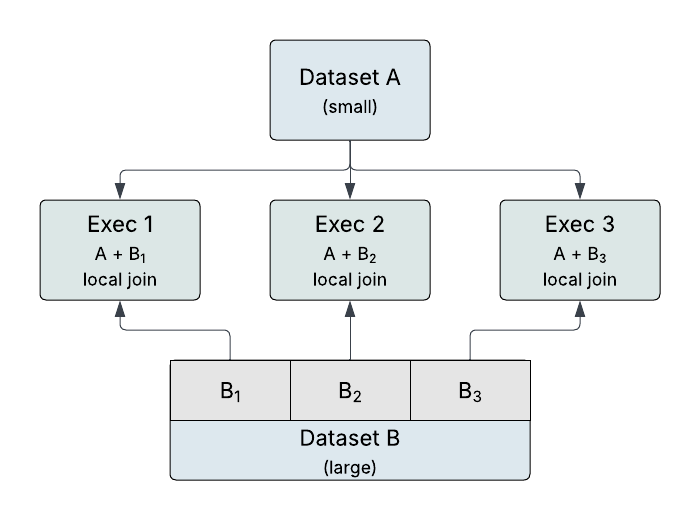
\includegraphics[valign=t, width=0.45\textwidth]{Chapters/02-background/sub-chapters/figures/02-broadcast-join.png}%
	}
	\hfill
	\subfloat[Partitioned join.\label{fig:partitioned-join}]{%
		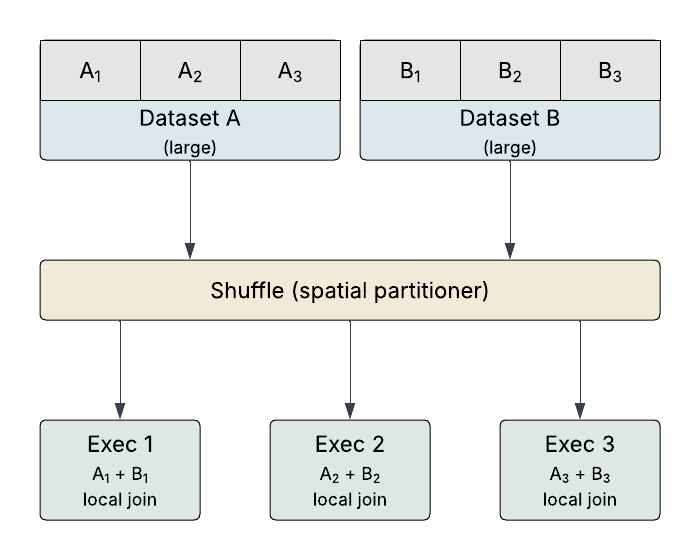
\includegraphics[valign=t, width=0.45\textwidth]{Chapters/02-background/sub-chapters/figures/02-partitioned-join.png}%
	}
	\caption[Broadcast versus partitioned spatial join]{Broadcast versus partitioned spatial join on the same two inputs. Both strategies converge on the same end state, three executors each performing a local join, but they differ sharply in where the network cost falls. (a) Broadcast: the small input A is shipped from a single source down to every executor; B's partitions are already resident on the executors and do not move, so network traffic scales only with the size of A. (b) Partitioned: both A and B flow through a shuffle that applies a common spatial partitioner, so spatially matching cells of A and B co-locate on each executor before the local join runs. Both inputs traverse the network in this case, and the heavy traffic is the cost of guaranteeing co-location.}
	\label{fig:broadcast-vs-partitioned-join}
\end{figure}

% \subsection{Apache Sedona}
% \label{subsec:sedona}
% Apache Sedona, formerly GeoSpark, is an open-source implementation of the spatial extensions described above. \textcite{yu2015_geospark_cluster_computing} introduced it as a Spark extension built around a new abstraction, the \acrfull{srdd}. The system matured through subsequent GeoSpark work, culminating in the comprehensive GeoInformatica reference description by \textcite{yu2019_geospark_perspective_beyond}. SpatialHadoop established this layered design on MapReduce, adding a spatial type system and operators to the distributed engine \parencite{eldawy2015_spatialhadoop_mapreduce_spatial}. Sedona adopts the same structure on Spark, exploiting Spark's in-memory data sharing across operations \parencite{zaharia2012_resilient_distributed_datasets}.

% First, it adds a user-defined Geometry type to Spark \acrshort{sql} \parencite{sedona2024_spatial_sql_application}. Second, it provides a library of spatial functions, exposing functions such as \texttt{ST\_Contains}, \texttt{ST\_Intersects}, and \texttt{ST\_GeomFromWKT} \parencite{sedona2024_spatial_sql_application}. Third, it implements the spatial partitioners and per-partition indexes discussed in Section \ref{background:distributed-spatial-processing:spatial-partitioning-and-parallel-efficiency}, supporting KDB-Tree, Quad-Tree, and R-Tree partitioning together with Quad-Tree and R-Tree local indexes \parencite{sedona2024_spatial_rdd_application}. Fourth, it integrates with Catalyst \parencite{yu2019_geospark_perspective_beyond}, making these capabilities available through both the \acrshort{srdd} \acrshort{api} and the higher-level Sedona \acrshort{sql}/DataFrame \acrshort{api} \parencite{sedona2024_spatial_rdd_application,sedona2024_spatial_sql_application}. Figure \ref{fig:sedona-architecture-on-spark} situates these four features within Sedona's layered design over Spark Core.

% \begin{figure}[H]
% 	\centering
% 	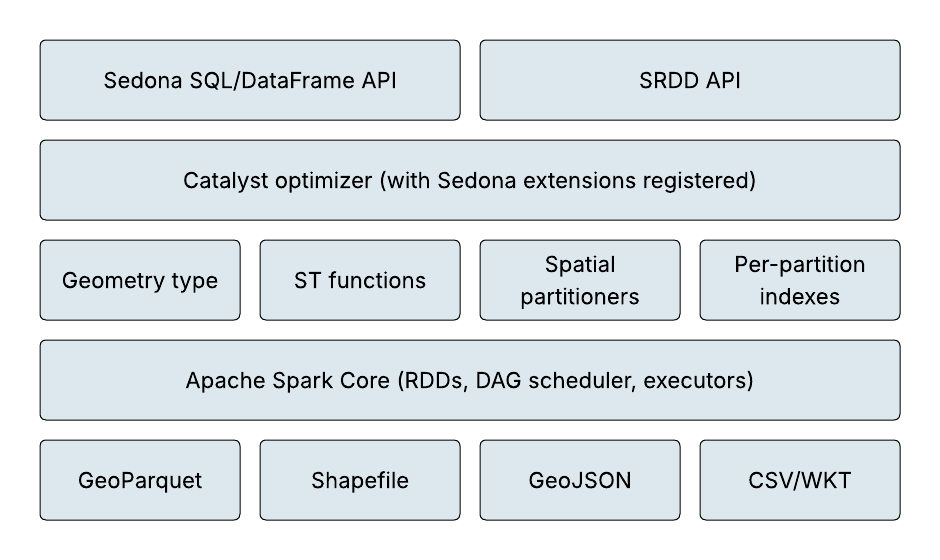
\includegraphics[width=0.7\textwidth]{Chapters/02-background/sub-chapters/figures/02-sedona-architecture-on-spark.png}
% 	\caption[Apache Sedona architecture on Apache Spark]{Layered architecture of Apache Sedona on Apache Spark. From top to bottom: two user-facing APIs (Sedona SQL/DataFrame and SRDD); the Catalyst optimizer with Sedona's \acrlong{udf}s~(\acrshort{udf}) and types registered; the four spatial extensions enumerated in the surrounding paragraph (Geometry type, ST functions, spatial partitioners, per-partition indexes); the Apache Spark runtime; and the storage formats Sedona reads directly. Adapted from \parencite{yu2015_geospark_cluster_computing}.}
% 	\label{fig:sedona-architecture-on-spark}
% \end{figure}

% Direct GeoParquet support is the feature that makes Sedona a suitable point of comparison for cloud-native query engines. Sedona reads the per-file bounding-box metadata defined by the GeoParquet specification and uses it to discard files whose extent cannot satisfy a spatial predicate, reducing the number of files scanned when the dataset is partitioned by spatial proximity \parencite{sedona2024_geoparquet_loader}. The combination of \acrshort{srdd}s, ST functions, spatial partitioners, and GeoParquet readers makes Sedona directly comparable to DuckDB on GeoParquet at the data-format level, while the underlying Spark run-time supplies the distributed lifecycle described in Section \ref{background:distributed-spatial-processing:the-lifecycle-of-a-distributed-spatial-query}.

\subsection{Apache Sedona}
\label{background:distributed-spatial-processing:apache-sedona}
Apache Sedona, formerly GeoSpark, is an open-source library that realizes the spatial extensions discussed in the preceding subsections on Apache Spark. \textcite{yu2015_geospark_cluster_computing} introduced it as a Spark extension built around a new abstraction, the \acrfull{srdd}, and later GeoSpark work consolidated the design in the GeoInformatica reference description by \textcite{yu2019_geospark_perspective_beyond}. The same layered design appeared earlier in SpatialHadoop, an analogous extension that added a spatial type system and operators to the Hadoop MapReduce engine, the batch-parallel paradigm that preceded Spark \parencite{eldawy2015_spatialhadoop_mapreduce_spatial}. Sedona adopts that structure on Spark and exploits Spark's in-memory data sharing across operations \parencite{zaharia2012_resilient_distributed_datasets}.

Sedona contributes four spatial extensions to the Spark engine. First, it adds a user-defined Geometry type to Spark \acrshort{sql} \parencite{sedona2024_spatial_sql_application}. Second, it provides a library of spatial functions, including \texttt{ST\_Contains}, \texttt{ST\_Intersects}, and \texttt{ST\_GeomFromWKT} \parencite{sedona2024_spatial_sql_application}. Third, it implements the spatial partitioners and per-partition indexes discussed in Section \ref{background:distributed-spatial-processing:spatial-partitioning-and-parallel-efficiency}, supporting KDB-Tree, Quad-Tree, and R-Tree partitioning together with Quad-Tree and R-Tree local indexes \parencite{sedona2024_spatial_rdd_application}. Fourth, it integrates with Catalyst \parencite{yu2019_geospark_perspective_beyond}, exposing these capabilities through both the \acrshort{srdd} \acrshort{api} and the higher-level Sedona \acrshort{sql}/DataFrame \acrshort{api} \parencite{sedona2024_spatial_rdd_application,sedona2024_spatial_sql_application}. Figure \ref{fig:sedona-architecture-on-spark} situates these four features within Sedona's layered design over Spark Core.

\begin{figure}[H]
	\centering
	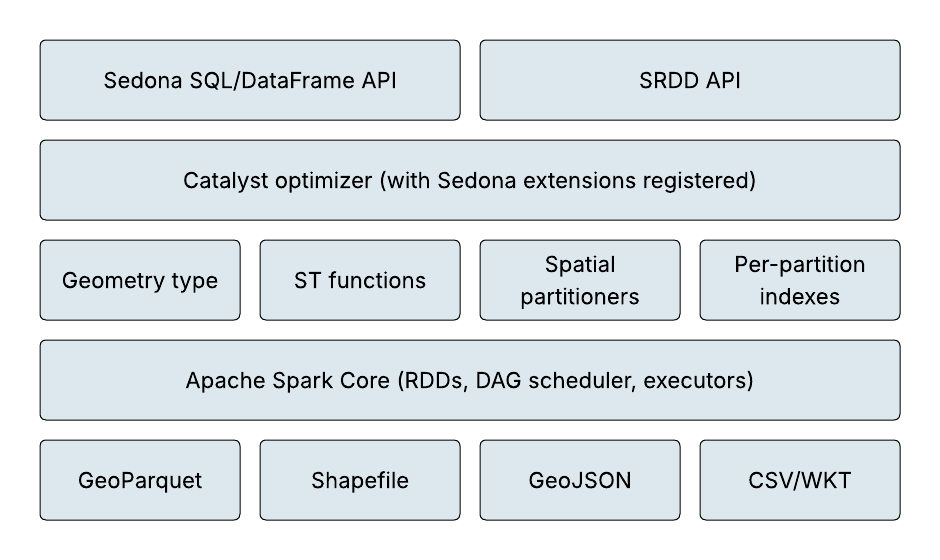
\includegraphics[width=0.7\textwidth]{Chapters/02-background/sub-chapters/figures/02-sedona-architecture-on-spark.png}
	\caption[Apache Sedona architecture on Apache Spark]{Layered architecture of Apache Sedona on Apache Spark. From top to bottom: two user-facing APIs (Sedona SQL/DataFrame and SRDD); the Catalyst optimizer with Sedona's \acrlong{udf}s~(\acrshort{udf}) and types registered; the four spatial extensions enumerated in the surrounding paragraph (Geometry type, ST functions, spatial partitioners, per-partition indexes); the Apache Spark runtime; and the storage formats Sedona reads directly. Adapted from \parencite{yu2015_geospark_cluster_computing}.}
	\label{fig:sedona-architecture-on-spark}
\end{figure}

Direct GeoParquet support is the feature that makes Sedona a suitable point of comparison for cloud-native query engines. Sedona reads the per-file bounding-box metadata defined by the GeoParquet specification and uses it to discard files whose extent cannot satisfy a spatial predicate, reducing the number of files scanned when the dataset is partitioned by spatial proximity \parencite{sedona2024_geoparquet_loader}. The combination of \acrshort{srdd}s, ST functions, spatial partitioners, and GeoParquet readers makes Sedona directly comparable to DuckDB on GeoParquet at the data-format level, while the underlying Spark run-time supplies the distributed lifecycle described in Section \ref{background:distributed-spatial-processing:the-lifecycle-of-a-distributed-spatial-query}.

% \subsection{Databricks as a Sedona run-time}
% \label{subsec:databricks}
% Apache Sedona is a library, not a managed service: it extends Apache Spark with distributed spatial datasets and functions, and therefore runs only inside an existing Spark cluster \parencite{sedona2026_sedonaspark}. Several run-time properties of the Databricks-managed Spark platform shape how a Sedona job behaves on Azure, independently of Sedona itself, and matter when interpreting elapsed time and cost on this platform. Four such properties together determine the cost of a Sedona run beyond the cost of the query itself: cluster startup, autoscaling, the separation of compute from storage, and node-hour billing.

% A Databricks cluster consists of a driver node and zero or more worker nodes, each backed by a cloud-provider VM that must be acquired and initialized before any task runs \parencite{databricks2024_compute_configuration}. Databricks documents that classic compute has longer startup times than serverless \parencite{databricks2024_cost_optimization_best_practices}, during which the cloud provider bills for the underlying VMs even when no workload is running \parencite{databricks2024_pool_index}. For short queries, this provisioning interval can dominate wall-clock time \parencite{databricks2024_cost_optimization_best_practices}.

% Autoscaling controls the number of executors actively billed during a job \parencite{databricks2024_compute_configuration}. Databricks's optimized autoscaler tracks idle executors and removes them when work has drained, even mid-job \parencite{databricks2018_optimized_autoscaling}. Autoscaling decisions are made at a polling interval \parencite{databricks2024_compute_configuration}, so a burst of work that completes within that interval will not see additional executors provisioned. As a result, two runs of the same query on the same nominal cluster configuration can encounter different effective parallelism depending on whether the autoscaler has settled \parencite{databricks2018_optimized_autoscaling, databricks2024_compute_configuration}.

% A Databricks cluster reads data from external object storage over the network rather than from cluster-local disks~\parencite{databricks2025_lakehouse, pang2024_storage_disaggregated_databases}. Every cold read therefore crosses the network between compute and storage \parencite{pang2024_storage_disaggregated_databases}, and that cost is absorbed into the executor read time described in Section \ref{background:distributed-spatial-processing:the-lifecycle-of-a-distributed-spatial-query}.

% Databricks bills compute at per-second granularity~\parencite{databricks2024_pricing}. The cost of a Sedona run is therefore the product of the cluster size and its lifetime, including provisioning~\parencite{databricks2024_pool_index} and any post-job idle period before auto-termination~\parencite{databricks2024_compute_configuration}. The relationship between elapsed query time and billed compute time on this platform is therefore mediated by these run-time properties rather than determined by the query alone.

\subsection{Databricks as a Sedona run-time}
\label{background:distributed-spatial-processing:databricks-as-a-sedona-run-time}
Apache Sedona is a library rather than a managed service, extending Apache Spark with distributed spatial datasets and functions, and therefore runs only inside an existing Spark cluster \parencite{sedona2026_sedonaspark}. On Azure, Databricks, a managed Apache Spark service, supplies that cluster, and several run-time properties of the platform shape how a Sedona job behaves independently of Sedona itself, which matters when interpreting elapsed time and cost. Four such properties together determine the cost of a Sedona run beyond the cost of the query itself: cluster startup, autoscaling, the separation of compute from storage, and node-hour billing.

A Databricks cluster consists of a driver node and zero or more worker nodes, each backed by a cloud-provider \acrfull{vm}, a software-emulated computer the provider allocates from physical hardware, that must be acquired and initialized before any task runs \parencite{databricks2024_compute_configuration}. Databricks documents that classic compute, the non-serverless cluster mode in which the customer specifies the \acrshort{vm} type and count, has longer startup times than serverless \parencite{databricks2024_cost_optimization_best_practices}, during which the provider bills for the underlying \acrshort{vm}s even when no workload is running \parencite{databricks2024_pool_index}. For short queries, this provisioning interval can dominate wall-clock time \parencite{databricks2024_cost_optimization_best_practices}.

Autoscaling controls the number of executors actively billed during a job \parencite{databricks2024_compute_configuration}. Databricks's optimized autoscaler tracks idle executors and removes them when work has drained, even mid-job \parencite{databricks2018_optimized_autoscaling}. Decisions are made at a polling interval, a fixed cadence at which the autoscaler reassesses cluster load \parencite{databricks2024_compute_configuration}, so a burst of work that completes within that interval will not see additional executors provisioned. Two runs of the same query on the same nominal cluster configuration can therefore encounter different effective parallelism depending on whether the autoscaler has settled \parencite{databricks2018_optimized_autoscaling, databricks2024_compute_configuration}.

A Databricks cluster reads data from external object storage over the network rather than from cluster-local disks \parencite{databricks2025_lakehouse, pang2024_storage_disaggregated_databases}. Every cold read, a read against data not already cached on the executor, therefore crosses the network between compute and storage \parencite{pang2024_storage_disaggregated_databases}, and that cost is absorbed into the executor read time described in Section \ref{background:distributed-spatial-processing:the-lifecycle-of-a-distributed-spatial-query}.

Databricks bills compute at per-second granularity \parencite{databricks2024_pricing}. The cost of a Sedona run is the product of cluster size and lifetime, including the provisioning interval \parencite{databricks2024_pool_index} and any post-job idle period before auto-termination \parencite{databricks2024_compute_configuration}. Elapsed query time and billed compute time on this platform are therefore mediated by these run-time properties rather than determined by the query alone.

% \subsection{Summary}
% \label{subsec:dist-summary}
% A distributed spatial query follows a fixed lifecycle: driver-side planning, parallel reads from object storage, narrow stages pipelined within executors, wide stages separated by shuffles, and a final action that writes results or collects them on the driver. Whether this lifecycle parallelizes depends on a spatial partitioner that co-locates nearby geometries, a per-partition local index that accelerates the local work, and the absence of skew that would funnel work onto a single straggler. Range queries run within a single stage, while spatial joins cross a stage boundary and are resolved via either broadcast or partitioned execution. Apache Sedona provides the spatial types, functions, partitioners, and GeoParquet readers needed to express these operations as Spark \acrshort{sql} queries, while Databricks provides the cluster lifecycle, autoscaling, and object storage connectivity that make Sedona a running service.

\subsection{Summary}
\label{background:distributed-spatial-processing:summary}
A distributed spatial query follows a fixed lifecycle: driver-side planning, parallel reads from object storage, narrow stages pipelined within executors, wide stages separated by shuffles, and a final action that writes results or collects them on the driver. The lifecycle parallelizes only when three conditions hold: a spatial partitioner co-locates nearby geometries, a per-partition local index accelerates the work within each partition, and skew does not funnel work onto a single straggler. Range queries run within a single stage; spatial joins cross a stage boundary and resolve through either broadcast or partitioned execution. Apache Sedona supplies the spatial types, functions, partitioners, and GeoParquet readers that express these operations as Spark \acrshort{sql} queries. Databricks supplies the cluster lifecycle, autoscaling, and object storage connectivity that make Sedona a running service.